% Options for packages loaded elsewhere
\PassOptionsToPackage{unicode}{hyperref}
\PassOptionsToPackage{hyphens}{url}
%
\documentclass[
  11pt,
  letterpaper,
]{book}

\usepackage{amsmath,amssymb}
\usepackage{lmodern}
\usepackage{iftex}
\ifPDFTeX
  \usepackage[T1]{fontenc}
  \usepackage[utf8]{inputenc}
  \usepackage{textcomp} % provide euro and other symbols
\else % if luatex or xetex
  \usepackage{unicode-math}
  \defaultfontfeatures{Scale=MatchLowercase}
  \defaultfontfeatures[\rmfamily]{Ligatures=TeX,Scale=1}
\fi
% Use upquote if available, for straight quotes in verbatim environments
\IfFileExists{upquote.sty}{\usepackage{upquote}}{}
\IfFileExists{microtype.sty}{% use microtype if available
  \usepackage[]{microtype}
  \UseMicrotypeSet[protrusion]{basicmath} % disable protrusion for tt fonts
}{}
\makeatletter
\@ifundefined{KOMAClassName}{% if non-KOMA class
  \IfFileExists{parskip.sty}{%
    \usepackage{parskip}
  }{% else
    \setlength{\parindent}{0pt}
    \setlength{\parskip}{6pt plus 2pt minus 1pt}}
}{% if KOMA class
  \KOMAoptions{parskip=half}}
\makeatother
\usepackage{xcolor}
\setlength{\emergencystretch}{3em} % prevent overfull lines
\setcounter{secnumdepth}{5}
% Make \paragraph and \subparagraph free-standing
\ifx\paragraph\undefined\else
  \let\oldparagraph\paragraph
  \renewcommand{\paragraph}[1]{\oldparagraph{#1}\mbox{}}
\fi
\ifx\subparagraph\undefined\else
  \let\oldsubparagraph\subparagraph
  \renewcommand{\subparagraph}[1]{\oldsubparagraph{#1}\mbox{}}
\fi

\usepackage{color}
\usepackage{fancyvrb}
\newcommand{\VerbBar}{|}
\newcommand{\VERB}{\Verb[commandchars=\\\{\}]}
\DefineVerbatimEnvironment{Highlighting}{Verbatim}{commandchars=\\\{\}}
% Add ',fontsize=\small' for more characters per line
\usepackage{framed}
\definecolor{shadecolor}{RGB}{241,243,245}
\newenvironment{Shaded}{\begin{snugshade}}{\end{snugshade}}
\newcommand{\AlertTok}[1]{\textcolor[rgb]{0.68,0.00,0.00}{#1}}
\newcommand{\AnnotationTok}[1]{\textcolor[rgb]{0.37,0.37,0.37}{#1}}
\newcommand{\AttributeTok}[1]{\textcolor[rgb]{0.40,0.45,0.13}{#1}}
\newcommand{\BaseNTok}[1]{\textcolor[rgb]{0.68,0.00,0.00}{#1}}
\newcommand{\BuiltInTok}[1]{\textcolor[rgb]{0.00,0.23,0.31}{#1}}
\newcommand{\CharTok}[1]{\textcolor[rgb]{0.13,0.47,0.30}{#1}}
\newcommand{\CommentTok}[1]{\textcolor[rgb]{0.37,0.37,0.37}{#1}}
\newcommand{\CommentVarTok}[1]{\textcolor[rgb]{0.37,0.37,0.37}{\textit{#1}}}
\newcommand{\ConstantTok}[1]{\textcolor[rgb]{0.56,0.35,0.01}{#1}}
\newcommand{\ControlFlowTok}[1]{\textcolor[rgb]{0.00,0.23,0.31}{#1}}
\newcommand{\DataTypeTok}[1]{\textcolor[rgb]{0.68,0.00,0.00}{#1}}
\newcommand{\DecValTok}[1]{\textcolor[rgb]{0.68,0.00,0.00}{#1}}
\newcommand{\DocumentationTok}[1]{\textcolor[rgb]{0.37,0.37,0.37}{\textit{#1}}}
\newcommand{\ErrorTok}[1]{\textcolor[rgb]{0.68,0.00,0.00}{#1}}
\newcommand{\ExtensionTok}[1]{\textcolor[rgb]{0.00,0.23,0.31}{#1}}
\newcommand{\FloatTok}[1]{\textcolor[rgb]{0.68,0.00,0.00}{#1}}
\newcommand{\FunctionTok}[1]{\textcolor[rgb]{0.28,0.35,0.67}{#1}}
\newcommand{\ImportTok}[1]{\textcolor[rgb]{0.00,0.46,0.62}{#1}}
\newcommand{\InformationTok}[1]{\textcolor[rgb]{0.37,0.37,0.37}{#1}}
\newcommand{\KeywordTok}[1]{\textcolor[rgb]{0.00,0.23,0.31}{#1}}
\newcommand{\NormalTok}[1]{\textcolor[rgb]{0.00,0.23,0.31}{#1}}
\newcommand{\OperatorTok}[1]{\textcolor[rgb]{0.37,0.37,0.37}{#1}}
\newcommand{\OtherTok}[1]{\textcolor[rgb]{0.00,0.23,0.31}{#1}}
\newcommand{\PreprocessorTok}[1]{\textcolor[rgb]{0.68,0.00,0.00}{#1}}
\newcommand{\RegionMarkerTok}[1]{\textcolor[rgb]{0.00,0.23,0.31}{#1}}
\newcommand{\SpecialCharTok}[1]{\textcolor[rgb]{0.37,0.37,0.37}{#1}}
\newcommand{\SpecialStringTok}[1]{\textcolor[rgb]{0.13,0.47,0.30}{#1}}
\newcommand{\StringTok}[1]{\textcolor[rgb]{0.13,0.47,0.30}{#1}}
\newcommand{\VariableTok}[1]{\textcolor[rgb]{0.07,0.07,0.07}{#1}}
\newcommand{\VerbatimStringTok}[1]{\textcolor[rgb]{0.13,0.47,0.30}{#1}}
\newcommand{\WarningTok}[1]{\textcolor[rgb]{0.37,0.37,0.37}{\textit{#1}}}

\providecommand{\tightlist}{%
  \setlength{\itemsep}{0pt}\setlength{\parskip}{0pt}}\usepackage{longtable,booktabs,array}
\usepackage{calc} % for calculating minipage widths
% Correct order of tables after \paragraph or \subparagraph
\usepackage{etoolbox}
\makeatletter
\patchcmd\longtable{\par}{\if@noskipsec\mbox{}\fi\par}{}{}
\makeatother
% Allow footnotes in longtable head/foot
\IfFileExists{footnotehyper.sty}{\usepackage{footnotehyper}}{\usepackage{footnote}}
\makesavenoteenv{longtable}
\usepackage{graphicx}
\makeatletter
\def\maxwidth{\ifdim\Gin@nat@width>\linewidth\linewidth\else\Gin@nat@width\fi}
\def\maxheight{\ifdim\Gin@nat@height>\textheight\textheight\else\Gin@nat@height\fi}
\makeatother
% Scale images if necessary, so that they will not overflow the page
% margins by default, and it is still possible to overwrite the defaults
% using explicit options in \includegraphics[width, height, ...]{}
\setkeys{Gin}{width=\maxwidth,height=\maxheight,keepaspectratio}
% Set default figure placement to htbp
\makeatletter
\def\fps@figure{htbp}
\makeatother

\setkeys{Gin}{width=\linewidth,height=\textheight,keepaspectratio}
% \usepackage[mathscr]{eucal}
\DeclareMathAlphabet{\mathscr}{U}{rsfs}{m}{n}

% \DeclareMathAlphabet{\mathcal}{OMS}{cmsy}{m}{n}
\usepackage{booktabs}
\usepackage[left=1.2in, right= 1.2in]{geometry}
\makeatletter
\def\thm@space@setup{%
  \thm@preskip=8pt plus 2pt minus 4pt
  \thm@postskip=\thm@preskip
}
\makeatother

% \AtBeginDocument{

% \geometry{left=1.2in, right= 1.2in}
\usepackage{fourier}
\usepackage[french]{babel}
\usepackage{tabu}
% \usepackage{animate}
% }

\newcommand{\bs}[1]{\boldsymbol{#1}}
\newcommand{\eps}{\varepsilon}
\newcommand{\Rlang}{\textsf{R}}
\newcommand{\SAS}{\textsf{SAS}}
\newcommand{\Sp}{\mathscr{S}}
\renewcommand{\P}[1]{{\mathsf P}\left(#1\right)}
\newcommand{\E}[1]{{\mathsf E}\left(#1\right)}
\newcommand{\Va}[1]{{\mathsf{Var}}\left(#1\right)}
\newcommand{\Cor}[1]{{\mathsf{Cor}}\left(#1\right)}
\newcommand{\I}[1]{{\mathbf 1}_{#1}}
\newcommand{\expit}{\mathrm{expit}}
\newcommand{\logit}{\mathrm{logit}}
\newcommand{\code}[1]{\texttt{#1}}
\newcommand{\Hy}{\mathcal{H}}
\renewcommand{\d}{\mathrm{d}}
\usepackage{booktabs}
\usepackage{longtable}
\usepackage{array}
\usepackage{multirow}
\usepackage{wrapfig}
\usepackage{float}
\usepackage{colortbl}
\usepackage{pdflscape}
\usepackage{tabu}
\usepackage{threeparttable}
\usepackage{threeparttablex}
\usepackage[normalem]{ulem}
\usepackage{makecell}
\usepackage{xcolor}
\makeatletter
\@ifpackageloaded{tcolorbox}{}{\usepackage[many]{tcolorbox}}
\@ifpackageloaded{fontawesome5}{}{\usepackage{fontawesome5}}
\definecolor{quarto-callout-color}{HTML}{909090}
\definecolor{quarto-callout-note-color}{HTML}{0758E5}
\definecolor{quarto-callout-important-color}{HTML}{CC1914}
\definecolor{quarto-callout-warning-color}{HTML}{EB9113}
\definecolor{quarto-callout-tip-color}{HTML}{00A047}
\definecolor{quarto-callout-caution-color}{HTML}{FC5300}
\definecolor{quarto-callout-color-frame}{HTML}{acacac}
\definecolor{quarto-callout-note-color-frame}{HTML}{4582ec}
\definecolor{quarto-callout-important-color-frame}{HTML}{d9534f}
\definecolor{quarto-callout-warning-color-frame}{HTML}{f0ad4e}
\definecolor{quarto-callout-tip-color-frame}{HTML}{02b875}
\definecolor{quarto-callout-caution-color-frame}{HTML}{fd7e14}
\makeatother
\makeatletter
\makeatother
\makeatletter
\@ifpackageloaded{caption}{}{\usepackage{caption}}
\AtBeginDocument{%
\ifdefined\contentsname
  \renewcommand*\contentsname{Table des matières}
\else
  \newcommand\contentsname{Table des matières}
\fi
\ifdefined\listfigurename
  \renewcommand*\listfigurename{Liste des figures}
\else
  \newcommand\listfigurename{Liste des figures}
\fi
\ifdefined\listtablename
  \renewcommand*\listtablename{Liste des tableaux}
\else
  \newcommand\listtablename{Liste des tableaux}
\fi
\ifdefined\figurename
  \renewcommand*\figurename{Figure}
\else
  \newcommand\figurename{Figure}
\fi
\ifdefined\tablename
  \renewcommand*\tablename{Tableau}
\else
  \newcommand\tablename{Tableau}
\fi
}
\@ifpackageloaded{float}{}{\usepackage{float}}
\floatstyle{ruled}
\@ifundefined{c@chapter}{\newfloat{codelisting}{h}{lop}}{\newfloat{codelisting}{h}{lop}[chapter]}
\floatname{codelisting}{Énumération}
\newcommand*\listoflistings{\listof{codelisting}{Liste des énumérations}}
\usepackage{amsthm}
\theoremstyle{definition}
\newtheorem{example}{Exemple}[chapter]
\theoremstyle{remark}
\renewcommand*{\proofname}{Preuve}
\newtheorem*{remark}{Remarque}
\newtheorem*{solution}{Solution}
\makeatother
\makeatletter
\@ifpackageloaded{caption}{}{\usepackage{caption}}
\@ifpackageloaded{subcaption}{}{\usepackage{subcaption}}
\makeatother
\makeatletter
\@ifpackageloaded{tcolorbox}{}{\usepackage[many]{tcolorbox}}
\makeatother
\makeatletter
\@ifundefined{shadecolor}{\definecolor{shadecolor}{rgb}{.97, .97, .97}}
\makeatother
\makeatletter
\makeatother
\ifLuaTeX
  \usepackage{selnolig}  % disable illegal ligatures
\fi
\IfFileExists{bookmark.sty}{\usepackage{bookmark}}{\usepackage{hyperref}}
\IfFileExists{xurl.sty}{\usepackage{xurl}}{} % add URL line breaks if available
\urlstyle{same} % disable monospaced font for URLs
\hypersetup{
  pdftitle={MATH 60602 - Analyse multidimensionnelle appliquée},
  pdfauthor={Denis Larocque; Léo Belzile},
  hidelinks,
  pdfcreator={LaTeX via pandoc}}

\title{MATH 60602 - Analyse multidimensionnelle appliquée}
\author{Denis Larocque \and Léo Belzile}
\date{avril 2022}

\begin{document}
\frontmatter
\maketitle
\ifdefined\Shaded\renewenvironment{Shaded}{\begin{tcolorbox}[boxrule=0pt, enhanced, interior hidden, frame hidden, sharp corners, borderline west={3pt}{0pt}{shadecolor}, breakable]}{\end{tcolorbox}}\fi

\renewcommand*\contentsname{Table des matières}
{
\setcounter{tocdepth}{2}
\tableofcontents
}
\mainmatter
\hypertarget{introduction}{%
\chapter{Introduction}\label{introduction}}

\hypertarget{survol-du-cours}{%
\section{Survol du cours}\label{survol-du-cours}}

\hypertarget{analyse-factorielle-exploratoire}{%
\subsection{Analyse factorielle
exploratoire}\label{analyse-factorielle-exploratoire}}

On dispose de \(p\) variables \(X_1, \ldots, X_p\). Peut-on expliquer
les interrelations (la structure de corrélation) entre ces variables à
l'aide d'un certain nombre (moins de \(p\)) de facteurs latents (non
observés)?

L'analyse factorielle est souvent utilisée pour analyser des
questionnaires (construction d'échelles) comme dans l'exemple suivant.

\leavevmode\vadjust pre{\hypertarget{exm-facto}{}}%
\begin{example}[]\label{exm-facto}

Pour les besoins d'une enquête, on a demandé à 200 consommateurs adultes
de répondre aux questions suivantes par rapport à un certain type de
magasin:

Sur une échelle de 1 à 5,

\begin{enumerate}
\def\labelenumi{\arabic{enumi}.}
\tightlist
\item
  pas important
\item
  peu important
\item
  moyennement important
\item
  assez important
\item
  très important
\end{enumerate}

Pour vous, à quel point est-ce important\ldots

\begin{enumerate}
\def\labelenumi{\arabic{enumi}.}
\tightlist
\item
  que le magasin offre de bons prix tous les jours?
\item
  que le magasin accepte les cartes de crédit majeures (Visa,
  Mastercard)?
\item
  que le magasin offre des produits de qualité?
\item
  que les vendeurs connaissent bien les produits?
\item
  qu'il y ait des ventes spéciales régulièrement?
\item
  que les marques connues soient disponibles?
\item
  que le magasin ait sa propre carte de crédit?
\item
  que le service soit rapide?
\item
  qu'il y ait une vaste sélection de produits?
\item
  que le magasin accepte le paiement par carte de débit?
\item
  que le personnel soit courtois?
\item
  que le magasin ait en stock les produits annoncés?
\end{enumerate}

Pouvons-nous identifier un nombre restreint de facteurs (concepts,
dimensions) qui pourraient bien rendre compte de la structure de
corrélation entre ces 12 variables?

\end{example}

Buts:

\begin{itemize}
\tightlist
\item
  Décrire et comprendre la structure de corrélation d'un ensemble de
  variables à l'aide d'un nombre restreint de concepts (appelés
  facteurs).
\item
  Réduire le nombre de variables en créant une nouvelle variable par
  facteur. Ces nouvelles variables pourront par la suite être utilisées
  dans d'autres analyses (régression linéaire multiple par exemple).
\end{itemize}

\hypertarget{analyse-de-regroupements}{%
\subsection{Analyse de regroupements}\label{analyse-de-regroupements}}

On cherche à créer des groupes (« \emph{clusters} ») d'individus
homogènes en utilisant \(p\) variables \(X_1, \ldots, X_p\).

Cette méthode est utilisée en marketing pour la \textbf{segmentation de
marché}, qui consiste en

\begin{quote}
\ldots définir des sous-groupes réunissant des consommateurs qui
partagent les mêmes préférences ou qui réagissent de façon semblable à
des variables de marketing\footnote{d'Astous, A. (2000). \emph{Le projet
  de recherche en marketing}, 2e édition. Chenelière/McGraw-Hill.}
\end{quote}

But:

\begin{itemize}
\tightlist
\item
  Combiner des sujets en groupes (interprétables) de telle sorte que les
  individus d'un même groupe soient les plus semblables possible par
  rapport à certaines caractéristiques et que les groupes soient les
  plus différents possible.
\end{itemize}

\hypertarget{suxe9lection-de-variables-et-de-moduxe8les}{%
\subsection{Sélection de variables et de
modèles}\label{suxe9lection-de-variables-et-de-moduxe8les}}

Dans plusieurs situations, on doit développer un modèle de prévision.
Par exemple, on pourrait devoir développer un modèle pour:

\begin{itemize}
\tightlist
\item
  Détecter les faillites des clients (ou des entreprises)
\item
  Cibler les clients qui seront intéressés par une offre promotionnelle
\item
  Détecter les fraudes (par carte de crédit ou dans les rapports de
  revenus)
\item
  Prévoir si un client va nous quitter.
\end{itemize}

Il y a en général plusieurs variables explicatives potentielles, et
aussi plusieurs types de modèles possibles (régression linéaire, réseaux
de neurones, arbres de régression ou de classification, etc.). Dans ce
chapitre, nous verrons des principes généraux et des outils afin de
sélectionner des modèles performants, ou bien un sous-ensemble de
variables avec un bon pouvoir prévisionnel.

\hypertarget{ruxe9gression-logistique}{%
\subsection{Régression logistique}\label{ruxe9gression-logistique}}

On cherche à expliquer le comportement d'une variable binaire \(Y\)
(\(0-1\)), à l'aide de \(p\) variables quelconques \(X_1, \ldots, X_p\).

\leavevmode\vadjust pre{\hypertarget{exm-logistique}{}}%
\begin{example}[]\label{exm-logistique}

Une banque offre aux gens la possibilité de faire une demande de carte
de crédit en ligne en promettant une approbation (conditionnelle) en
quelques minutes seulement. Le tout est basé sur un modèle automatique
de classification qui décide d'accorder ou non la carte (\(Y=1\) ou
\(Y=0\)) en fonction des réponses fournies par les clients potentiels à
différentes questions comme: quel est votre revenu annuel brut
(\(X_1\)), avez-vous d'autres cartes de crédit (\(X_2\)), êtes-vous
locataire ou propriétaire (\(X_3\)), etc\ldots

\end{example}

Buts:

\begin{itemize}
\tightlist
\item
  Comprendre comment et dans quelle mesure les variables
  \(\boldsymbol{X}\) influencent la catégorie d'appartenance de \(Y\).
\item
  Développer un modèle pour faire de la classification, c'est-à-dire,
  prévoir la catégorie d'appartenance de \(Y\) pour un nouveau sujet à
  partir des variables \(\boldsymbol{X}\).
\end{itemize}

\hypertarget{analyse-de-survie}{%
\subsection{Analyse de survie}\label{analyse-de-survie}}

On s'intéresse au temps avant qu'un événement survienne. Par exemple :

\begin{itemize}
\tightlist
\item
  Temps qu'un client demeure abonné à un service offert par notre
  compagnie.
\item
  Temps de survie d'un individu après avoir été diagnostiqué avec un
  certain type de cancer.
\item
  Temps qu'un employé demeure au service de la compagnie.
\item
  Temps qu'une franchise demeure en activité.
\item
  Temps avant la faillite d'une entreprise (ou d'un particulier).
\item
  Temps avant le prochain achat d'un client.
\end{itemize}

On observe chaque sujet jusqu'à ce que l'une des deux choses suivantes
se produise: l'événement survient avant la fin de la période
d'observation ou bien l'étude se termine et l'événement n'est toujours
pas survenu. Dans le premier exemple, l'événement correspond au fait
d'interrompre son abonnement. On dispose donc d'une variable temps \(T\)
pour chaque individu qui est soit censurée, soit non censurée. Si
l'individu a expérimenté l'événement avant la fin de la période
d'observation, la valeur de est non censurée. Si l'événement n'est
toujours pas survenu à la fin de la période d'observation, la valeur de
\(T\) est censurée. Pour chaque individu, on dispose également d'un
ensemble de variables explicatives \(X_1, \ldots, X_p\).

But:

\begin{itemize}
\tightlist
\item
  Étudier les effets des variables explicatives sur le temps de survie
  et obtenir des prévisions du temps de survie.
\end{itemize}

\hypertarget{donnuxe9es-manquantes}{%
\subsection{Données manquantes}\label{donnuxe9es-manquantes}}

Il arrive fréquemment d'avoir des valeurs manquantes dans notre
échantillon.

Simplement ignorer les sujets avec des valeurs manquantes et faire
l'analyse avec les autres sujets conduit généralement à des estimations
biaisées et à de l'inférence invalide.

Dans ce chapitre, nous verrons une méthode très générale afin de traiter
les données manquantes, l'imputation multiple. Nous verrons comment elle
peut être utilisée dans un contexte d'inférence et dans un contexte de
prévision.

\hypertarget{analyse-exploratoire}{%
\chapter{Analyse exploratoire de données}\label{analyse-exploratoire}}

L'analyse exploratoire, comme son nom l'indique, est une étape
préliminaire à la modélisation servant à l'acquisition d'une meilleure
compréhension des données. L'analyse exploratoire sert à nous assurer
que notre analyse ou notre traitement de ces dernières est cohérent. Le
but de l'analyse exploratoire graphique est d'extraire des informations
utiles, le plus souvent par le biais d'une série de questions qui sont
raffinées au fur et à mesure que progresse l'analyse. On s'intéresse
particulièrement aux relations et interactions entre différentes
variables et la distribution empirique de chaque variable. Les étapes
majeures sont:

\begin{enumerate}
\def\labelenumi{\arabic{enumi}.}
\tightlist
\item
  Formuler des questions sur les données
\item
  Chercher des réponses à ces questions à l'aide de statistiques
  descriptives, de tableaux de fréquence ou de contingence et de
  graphiques.
\item
  Raffiner nos questions, et utiliser les trouvailles pour peaufiner
  notre analyse
\end{enumerate}

Dans un rapport, un résumé des caractéristiques les plus importantes
devrait être inclut pour que le lecteur ou la lectrice puisse valider
son interprétation des données.

\hypertarget{types-de-variables}{%
\section{Types de variables}\label{types-de-variables}}

\begin{itemize}
\tightlist
\item
  Une \textbf{variable} représente une caractéristique de la population
  d'intérêt, par exemple le sexe d'un individu, le prix d'un article,
  etc.
\item
  une \textbf{observation}, parfois appelée donnée, est un ensemble de
  mesures collectées sous des conditions identiques, par exemple pour un
  individu ou à un instant donné.
\end{itemize}

Le choix de modèle statistique ou de test dépend souvent du type de
variables collectées. Les variables peuvent être de plusieurs types:
quantitatives (discrètes ou continues) si elles prennent des valeurs
numériques, qualitatives (binaires, nominales ou ordinales) si elles
sont décrites par un adjectif; je préfère le terme catégorielle, plus
évocateur.

\begin{figure}

\begin{minipage}[t]{0.45\linewidth}

{\centering 

\raisebox{-\height}{

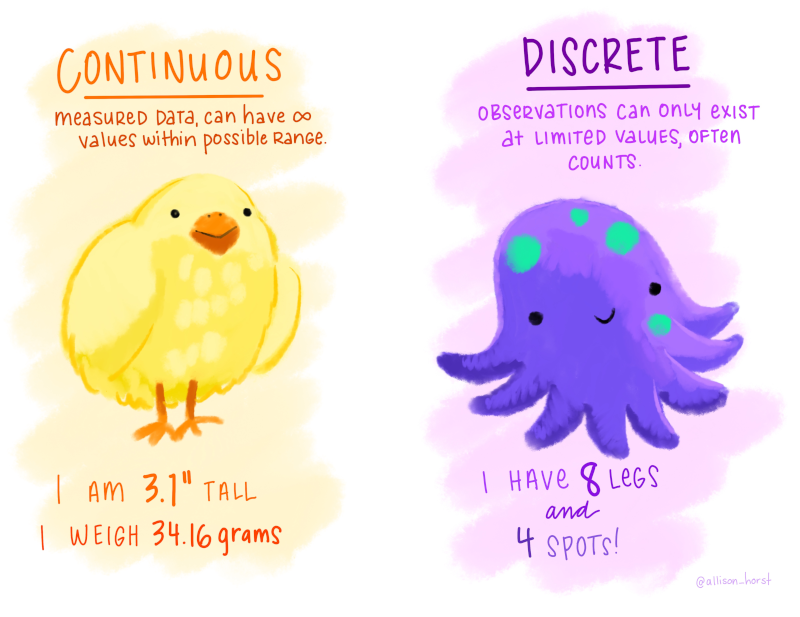
\includegraphics{./figures/continuous_discrete.png}

}

}

\end{minipage}%
%
\begin{minipage}[t]{0.55\linewidth}

{\centering 

\raisebox{-\height}{

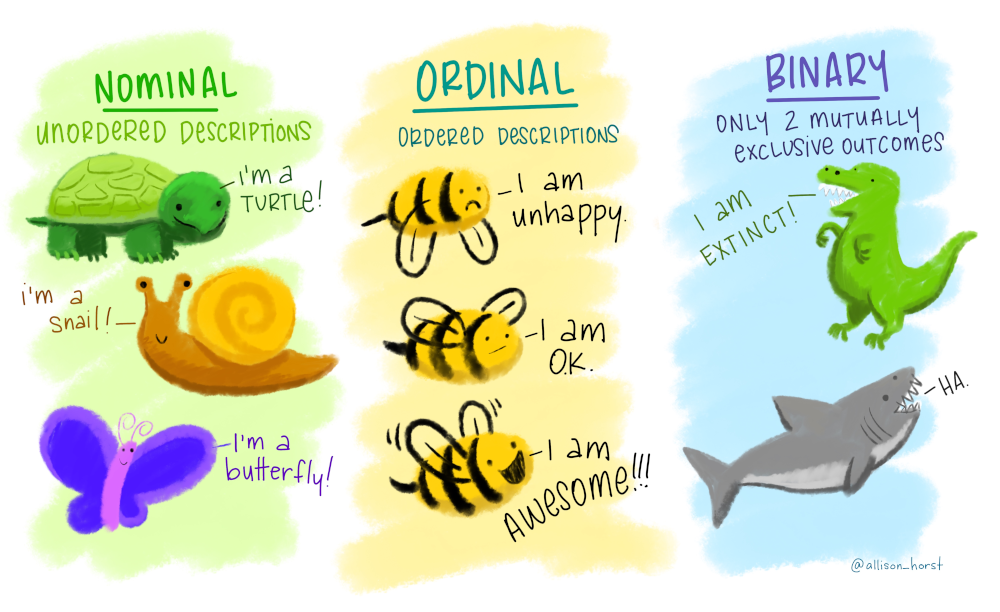
\includegraphics{./figures/nominal_ordinal_binary.png}

}

}

\end{minipage}%

\caption{\label{fig-types-variables}Illustrations par Allison Horst de
variables numériques (gauche) et catégorielles (droite).}

\end{figure}

On distingue deux types de variables quantitatives:

\begin{itemize}
\tightlist
\item
  une variable discrète prend un nombre dénombrable de valeurs; ce sont
  souvent des variables de dénombrement ou des variables dichotomiques.
\item
  une variable continue peut prendre (en théorie) une infinité de
  valeurs, même si les valeurs mesurées sont arrondies ou mesurées avec
  une précision limitée (temps, taille, masse, vitesse, salaire). Dans
  bien des cas, nous pouvons considérer comme continues des variables
  discrètes si elles prennent un assez grand nombre de valeurs.
\end{itemize}

Les variables catégorielles représentent un ensemble fini de
possibilités. On les regroupe en deux types, pour lesquels on ne fera
pas de distinction:

\begin{itemize}
\tightlist
\item
  nominales s'il n'y a pas d'ordre entre les modalités (sexe, couleur,
  pays d'origine) ou
\item
  ordinale (échelle de Likert, tranche salariale).
\end{itemize}

La codification des modalités des variables catégorielle est arbitraire;
en revanche, on préservera l'ordre lorsqu'on représentera graphiquement
les variables ordinales. Lors de l'estimation, chaque variable
catégorielle doit est transformée en un ensemble d'indicateurs binaires:
il est donc essentiel de déclarer ces dernières dans votre logiciel
statistique, surtout si elles sont encodées dans la base de données à
l'aide de valeurs entières.

\hypertarget{validation-des-donnuxe9es.}{%
\section{Validation des données.}\label{validation-des-donnuxe9es.}}

Avant de regarder les données, il est souvent utile de se plonger dans
la description de la base de données. Il n'est pas rare que cette
dernière contienne des informations pertinentes sur la codification des
données, par exemple

\begin{itemize}
\tightlist
\item
  telle variable catégorielle est stockée avec des valeurs entières et
  les étiquettes ne sont disponibles que dans la description.
\item
  des valeurs manquantes sont encodées avec \(-1\) (pour les variables
  positives) ou \(999\).
\item
  une variable est une fonction, transformation ou combinaison d'autres
  variables.
\end{itemize}

\hypertarget{graphiques}{%
\section{Graphiques}\label{graphiques}}

Le principal type de graphique pour représenter la distribution d'une
variable catégorielle est le diagramme en bâtons, dans lequel la
fréquence de chaque catégorie est présentée sur l'axe des ordonnées
(\(y\)) en fonction de la modalité, sur l'axe des abscisses (\(x\)), et
ordonnées pour des variables ordinales. Cette représentation est en tout
point supérieur au
\href{http://www.perceptualedge.com/articles/08-21-07.pdf}{diagramme en
camembert}, une engeance répandue qui devrait être honnie (notamment
parce que l'humain juge mal les différences d'aires, qu'une simple
rotation change la perception du graphique et qu'il est difficile de
mesurer les proportions) --- ce n'est pas de la tarte!

\begin{Shaded}
\begin{Highlighting}[]
\FunctionTok{library}\NormalTok{(ggplot2); }
\FunctionTok{library}\NormalTok{(poorman)}
\FunctionTok{library}\NormalTok{(patchwork)}
\FunctionTok{data}\NormalTok{(renfe, }\AttributeTok{package =} \StringTok{"hecmodstat"}\NormalTok{)}

\NormalTok{g1 }\OtherTok{\textless{}{-}} \FunctionTok{ggplot}\NormalTok{(}\AttributeTok{data =}\NormalTok{ renfe, }\FunctionTok{aes}\NormalTok{(}\AttributeTok{x =}\NormalTok{ classe)) }\SpecialCharTok{+} 
  \FunctionTok{geom\_bar}\NormalTok{() }\SpecialCharTok{+} 
  \FunctionTok{labs}\NormalTok{(}\AttributeTok{x =} \StringTok{"classe"}\NormalTok{, }\AttributeTok{y =} \StringTok{"dénombrement"}\NormalTok{)}
\NormalTok{g2 }\OtherTok{\textless{}{-}} \FunctionTok{ggplot}\NormalTok{(}\AttributeTok{data =}\NormalTok{ renfe, }\FunctionTok{aes}\NormalTok{(}\AttributeTok{x =}\NormalTok{ type)) }\SpecialCharTok{+} 
  \FunctionTok{geom\_bar}\NormalTok{() }\SpecialCharTok{+} 
  \FunctionTok{labs}\NormalTok{(}\AttributeTok{x =} \StringTok{"type de train"}\NormalTok{, }\AttributeTok{y =} \StringTok{"dénombrement"}\NormalTok{)}
\NormalTok{g1 }\SpecialCharTok{+}\NormalTok{ g2}
\end{Highlighting}
\end{Shaded}

\begin{figure}[ht!]

{\centering 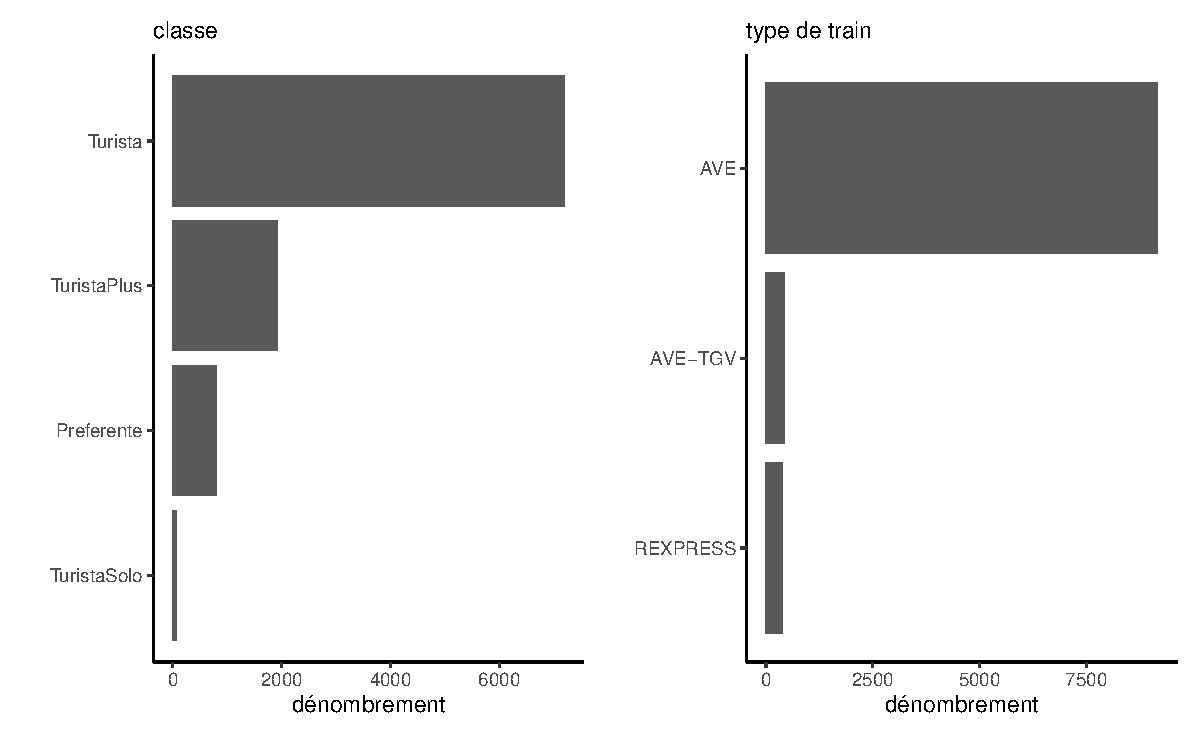
\includegraphics[width=1\textwidth,height=\textheight]{./01-analyseexploratoire_files/figure-pdf/fig-barplotrenfe-1.pdf}

}

\caption{\label{fig-barplotrenfe}Diagramme en bâtons pour la classe des
billets de trains du jeu de données Renfe.}

\end{figure}

Puisque les variables continues peuvent prendre autant de valeurs
distinctes qu'il y a d'observations, on ne peut simplement compter le
nombre d'occurrence par valeur unique. On regroupera plutôt dans un
certain nombre d'intervalle, en discrétisant l'ensemble des valeurs en
classes pour obtenir un histogramme. Le nombre de classes dépendra du
nombre d'observations si on veut que l'estimation ne soit pas impactée
par le faible nombre d'observations par classe: règle générale, le
nombre de classes ne devrait pas dépasser \(\sqrt{n}\), où \(n\) est le
nombre d'observations de l'échantillon. On obtiendra la fréquence de
chaque classe, mais si on normalise l'histogramme (de façon à ce que
l'aire sous les bandes verticales égale un), on obtient une
approximation discrète de la fonction de densité. Faire varier le nombre
de classes permet parfois de faire apparaître des caractéristiques de la
variable (notamment la multimodalité, l'asymmétrie et les arrondis).

Puisque qu'on groupe les observations en classe pour tracer
l'histogramme, il est difficile de voir l'étendue des valeurs que prenne
la variable: on peut rajouter des traits sous l'histogramme pour
représenter les valeurs uniques prises par la variable, tandis que la
hauteur de l'histogramme nous renseigne sur leur fréquence relative.

\begin{Shaded}
\begin{Highlighting}[]
\NormalTok{renfe }\SpecialCharTok{|\textgreater{}}
  \FunctionTok{subset}\NormalTok{(tarif }\SpecialCharTok{==} \StringTok{"Promo"}\NormalTok{) }\SpecialCharTok{|\textgreater{}}
  \FunctionTok{ggplot}\NormalTok{(}\FunctionTok{aes}\NormalTok{(}\AttributeTok{x =}\NormalTok{ prix)) }\SpecialCharTok{+} 
    \FunctionTok{geom\_histogram}\NormalTok{(}\FunctionTok{aes}\NormalTok{(}\AttributeTok{y =}\NormalTok{ ..density..), }
                   \AttributeTok{bins =} \DecValTok{30}\NormalTok{) }\SpecialCharTok{+}
    \FunctionTok{geom\_rug}\NormalTok{(}\AttributeTok{sides =} \StringTok{"b"}\NormalTok{) }\SpecialCharTok{+} 
    \FunctionTok{labs}\NormalTok{(}\AttributeTok{x =} \StringTok{"prix de billets au tarif Promo (en euros)"}\NormalTok{, }
         \AttributeTok{y =} \StringTok{"densité"}\NormalTok{) }
\end{Highlighting}
\end{Shaded}

\begin{figure}[ht!]

{\centering 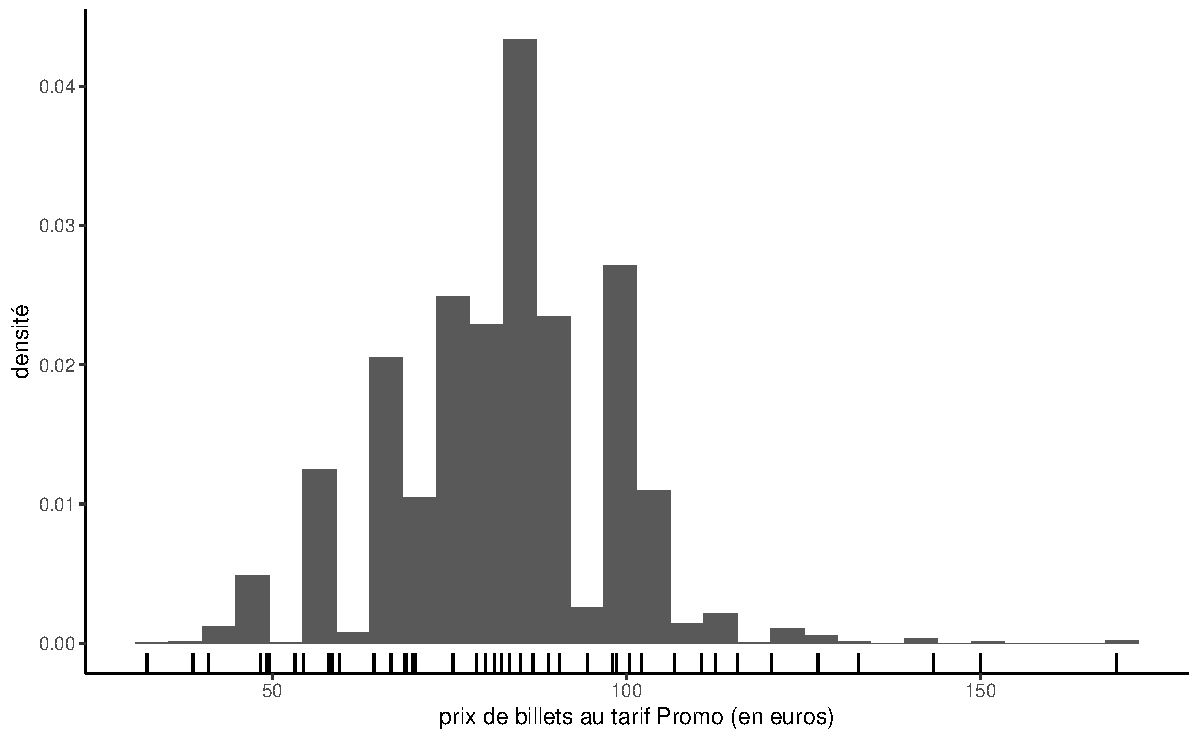
\includegraphics[width=1\textwidth,height=\textheight]{./01-analyseexploratoire_files/figure-pdf/fig-histrenfe-1.pdf}

}

\caption{\label{fig-histrenfe}Histogramme du prix des billets au tarif
Promo de trains du jeu de données Renfe}

\end{figure}

Une boîte à moustaches représente graphiquement cinq statistiques
descriptives.

\begin{itemize}
\tightlist
\item
  La boîte donne les 1e, 2e et 3e quartiles \(q_1, q_2, q_3\). Il y a
  donc 50\% des observations sont au-dessus/en-dessous de la médiane
  \(q_2\) qui sépare en deux la boîte.
\item
  La longueur des moustaches est moins de \(1.5\) fois l'écart
  interquartile \(q_3-q_1\) (tracée entre 3e quartile et le dernier
  point plus petit que \(q_3+1.5(q_3-q_1)\), etc.)
\item
  Les observations au-delà des moustaches sont encerclées. Notez que
  plus le nombre d'observations est élevé, plus le nombres de valeurs
  extrême augmente. C'est un défaut de la boîte à moustache, qui a été
  conçue pour des jeux de données qui passeraient pour petits selon les
  standards actuels.
\end{itemize}

\begin{figure}[ht!]

{\centering 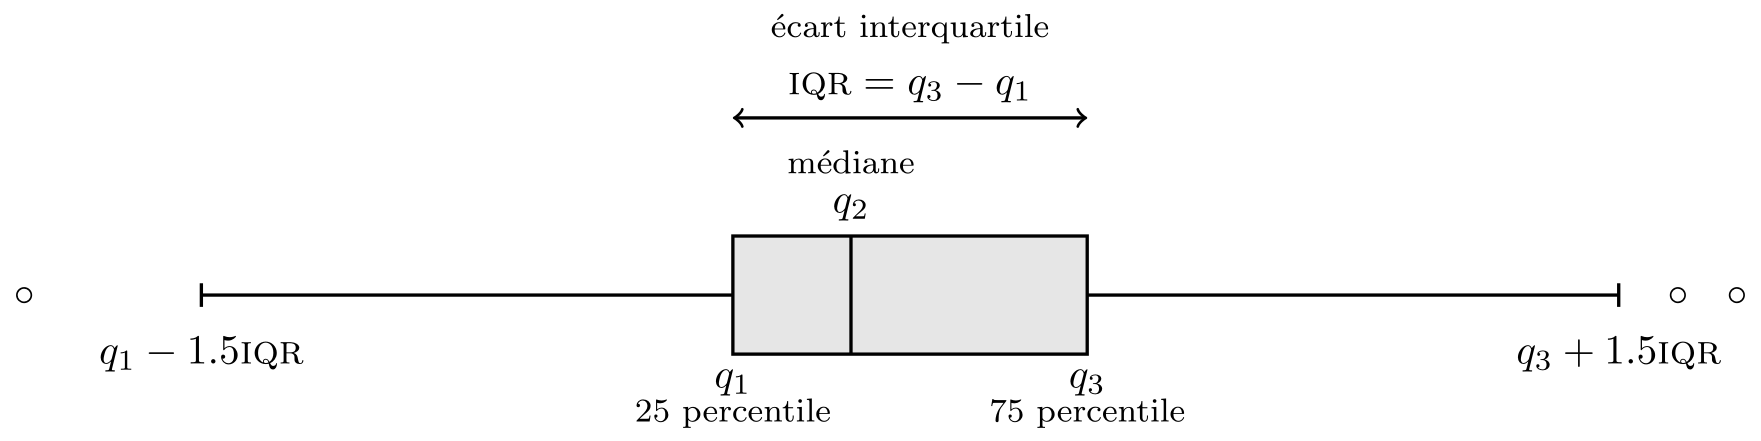
\includegraphics[width=1\textwidth,height=\textheight]{./figures/01-intro-boiteamoustache.png}

}

\caption{\label{fig-boiteamoustache}Boîte à moustache.}

\end{figure}

On peut représenter la distribution d'une variable réponse continue en
fonction d'une variable catégorielle en traçant une boîte à moustaches
pour chaque catégorie et en les disposant côte-à-côte. Une troisième
variable catégorielle peut être ajoutée par le biais de couleurs, comme
dans la Figure~\ref{fig-histboxplot}.

\begin{Shaded}
\begin{Highlighting}[]
\NormalTok{renfe }\SpecialCharTok{|\textgreater{}} 
   \FunctionTok{subset}\NormalTok{(tarif }\SpecialCharTok{==} \StringTok{"Promo"}\NormalTok{) }\SpecialCharTok{|\textgreater{}}
   \FunctionTok{ggplot}\NormalTok{(}\FunctionTok{aes}\NormalTok{(}\AttributeTok{y =}\NormalTok{ prix, }\AttributeTok{x =}\NormalTok{ classe, }\AttributeTok{col =}\NormalTok{ type)) }\SpecialCharTok{+} 
    \FunctionTok{geom\_boxplot}\NormalTok{() }\SpecialCharTok{+} 
    \FunctionTok{labs}\NormalTok{(}\AttributeTok{y =} \StringTok{"prix (en euros)"}\NormalTok{, }
         \AttributeTok{col =} \StringTok{"type de train"}\NormalTok{) }\SpecialCharTok{+} 
    \FunctionTok{theme}\NormalTok{(}\AttributeTok{legend.position =} \StringTok{"bottom"}\NormalTok{)}
\end{Highlighting}
\end{Shaded}

\begin{figure}[ht!]

{\centering 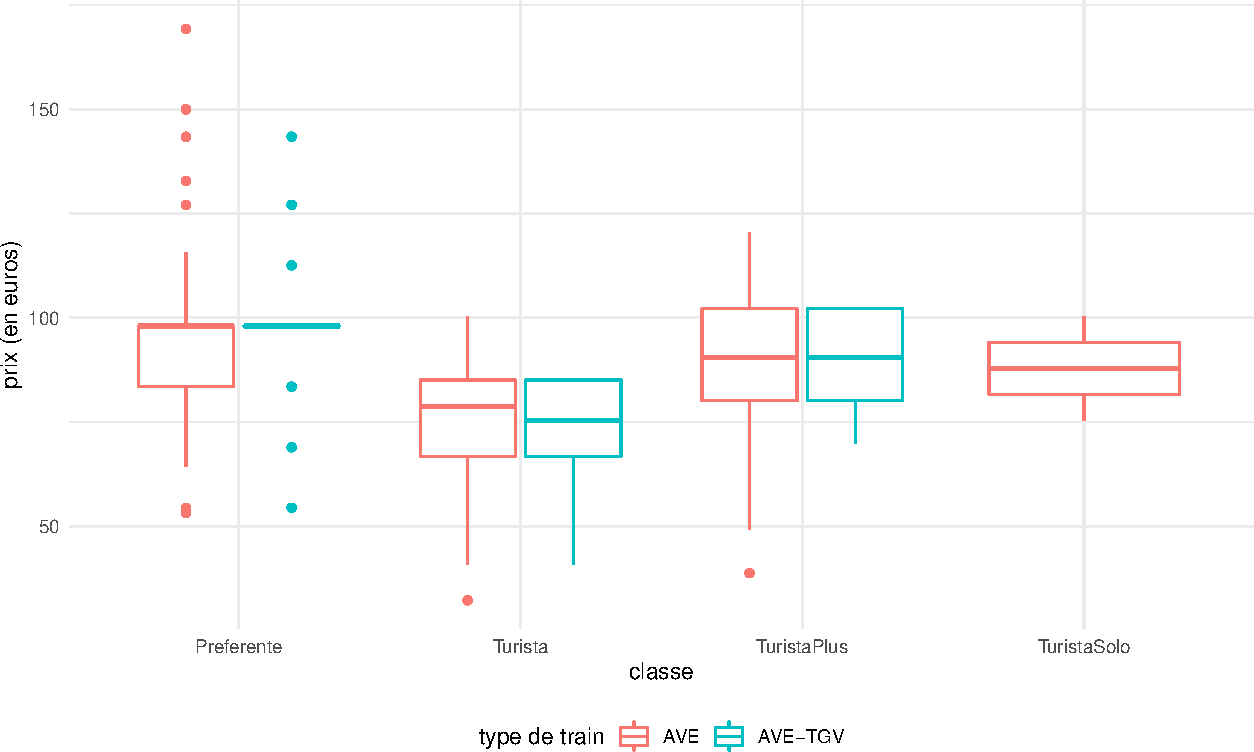
\includegraphics[width=1\textwidth,height=\textheight]{./01-analyseexploratoire_files/figure-pdf/fig-histboxplot-1.pdf}

}

\caption{\label{fig-histboxplot}Boîte à moustaches du prix des billets
au tarif Promo en fonction de la classe pour le jeu de données Renfe.}

\end{figure}

Si on veut représenter la covariabilité de deux variables continues, on
utilise un nuage de points où chaque variable est représentée sur un axe
et chaque observation donne la coordonnée des points. Si la
représentation graphique est dominée par quelques valeurs très grandes,
une transformation des données peut être utile: vous verrez souvent des
données positives à l'échelle logarithmique.

Plutôt que de décrire plus en détail le processus de l'analyse
exploratoire, on présente un exemple qui illustre le cheminement habitue
sur les données de trains de la Renfe introduites précédemment.

\hypertarget{analyse-exploratoire-des-billets-de-trains-renfe}{%
\section{Analyse exploratoire des billets de trains
Renfe}\label{analyse-exploratoire-des-billets-de-trains-renfe}}

La première étape consisterait à lire la description de la base de
données. Le jeu de données \texttt{renfe} contient les variables
suivantes:

\begin{itemize}
\tightlist
\item
  \texttt{prix}: prix du billet (en euros);
\item
  \texttt{dest}: indicateur binaire du trajet, soit de Barcelone vers
  Madrid (\texttt{0}) ou de Madrid vers Barcelone (\texttt{1});
\item
  \texttt{tarif}: variable catégorielle indiquant le tarif du billet, un
  parmi \texttt{AdultoIda}, \texttt{Promo} et \texttt{Flexible};
\item
  \texttt{classe}: classe du billet, soit \texttt{Preferente},
  \texttt{Turista}, \texttt{TuristaPlus} ou \texttt{TuristaSolo};
\item
  \texttt{type}: variable catégorielle indiquant le type de train, soit
  Alta Velocidad Española (\texttt{AVE}), soit Alta Velocidad Española
  conjointement avec TGV (un partenariat entre la SNCF et Renfe pour les
  trains à destination ou en provenance de Toulouse) \texttt{AVE-TGV},
  soit les trains régionaux \texttt{REXPRESS}; seuls les trains
  étiquetés \texttt{AVE} ou \texttt{AVE-TGV} sont des trains à grande
  vitesse.
\item
  \texttt{duree}: longueur annoncée du trajet (en minutes);
\item
  \texttt{jour} entier indiquant le jour de la semaine du départ allant
  de dimanche (\texttt{1}) à samedi (\texttt{7}).
\end{itemize}

Il n'y a pas de valeurs manquantes et un aperçu des données
(\texttt{head(renfe)}) montre qu'elles sont en format long, ce qui veut
dire que chaque ligne contient une seule valeur pour la variable
réponse, ici le prix d'un billet de train. On entame l'analyse
exploratoire avec des questions plutôt vagues, par exemple

\begin{enumerate}
\def\labelenumi{\arabic{enumi}.}
\tightlist
\item
  Quels sont les facteurs déterminant le prix et le temps de parcours?
\item
  Est-ce que le temps de parcours est le même peut importe le type de
  train?
\item
  Quelles sont les caractéristiques distinctives des types de train?
\item
  Quelles sont les principales différences entre les tarifs?
\end{enumerate}

À l'exception de \texttt{prix} et de \texttt{duree}, toutes les
variables explicatives sont catégorielles. La variable \texttt{jour}
prends des valeurs entre 1 et 7; s'en souvenir pour éviter les mauvaises
surprises ultérieures. En analysant le nombre de trains dans les
catégories, on remarque qu'il y a autant de billets de type
\texttt{REXPRESS} que le nombre de billets au tarif \texttt{AdultoIda}.
On peut faire le décompte par catégorie avec un tableau de contingence,
qui compte le nombre respectif dans chaque sous-catégorie. Dans la base
de données Renfe, tous les billets pour les RegioExpress sont vendus au
tarif \texttt{AdultoIda} en classe \texttt{Turista}. Le nombre de
billets est minime, à peine 397 sur 10000. Cela suggère une nouvelle
question: pourquoi ces trains sont-ils si peu populaires?

On remarque également que seulement 17 temps de parcours sont affichés
sur les billets. On peut donc penser que la durée affichée sur le billet
(en minutes) est le temps de trajet annoncé. La majeure partie (15 sur
17) des temps de parcours sont sous la barre des 3h15, hormis deux qui
dépassent les 9h! Selon Google Maps, les deux villes sont distantes de
615km par la route, 500km à vol d'oiseau. Cela implique que,
vraisemblablement, certains trains dépassent les 200km/h, tandis que
d'autres vont plutôt à 70km/h. Quels sont ces trains plus lent? La
variable \texttt{type} codifie probablement ce fait, et permet de voir
que ce sont les trains RegioExpress qui sont dans cette catégorie.

Aller de Madrid à Barcelone à l'aide d'un train régulier prend 18
minutes de plus. Avec plus de 9h de trajet, pas étonnant donc que ces
billets soient peu courus. Encore plus frappant, on note que le prix des
billets est fixe: 43.25 euros peu importe que le trajet soit aller ou
retour. C'est probablement la trouvaille la plus importante jusqu'à
maintenant, car les billets de train de type RegioExpress ne forment pas
un échantillon: il n'y a aucune variabilité! On aurait également pu
découvrir cette anomalie en traçant une boîte à moustaches du prix en
fonction du type de train.

\begin{Shaded}
\begin{Highlighting}[]
\FunctionTok{ggplot}\NormalTok{(}\AttributeTok{data =}\NormalTok{ renfe, }
       \AttributeTok{mapping =} \FunctionTok{aes}\NormalTok{(}\AttributeTok{x =}\NormalTok{ type, }\AttributeTok{y =}\NormalTok{ prix, }\AttributeTok{col =}\NormalTok{ dest)) }\SpecialCharTok{+} 
  \FunctionTok{geom\_boxplot}\NormalTok{() }\SpecialCharTok{+} 
  \FunctionTok{labs}\NormalTok{(}\AttributeTok{y =} \StringTok{"prix (en euros)"}\NormalTok{,}
       \AttributeTok{x =} \StringTok{"type de train"}\NormalTok{,}
       \AttributeTok{color =} \StringTok{"destination"}\NormalTok{) }\SpecialCharTok{+}
  \FunctionTok{theme}\NormalTok{(}\AttributeTok{legend.position =} \StringTok{"bottom"}\NormalTok{)}
\end{Highlighting}
\end{Shaded}

\begin{figure}[ht!]

{\centering 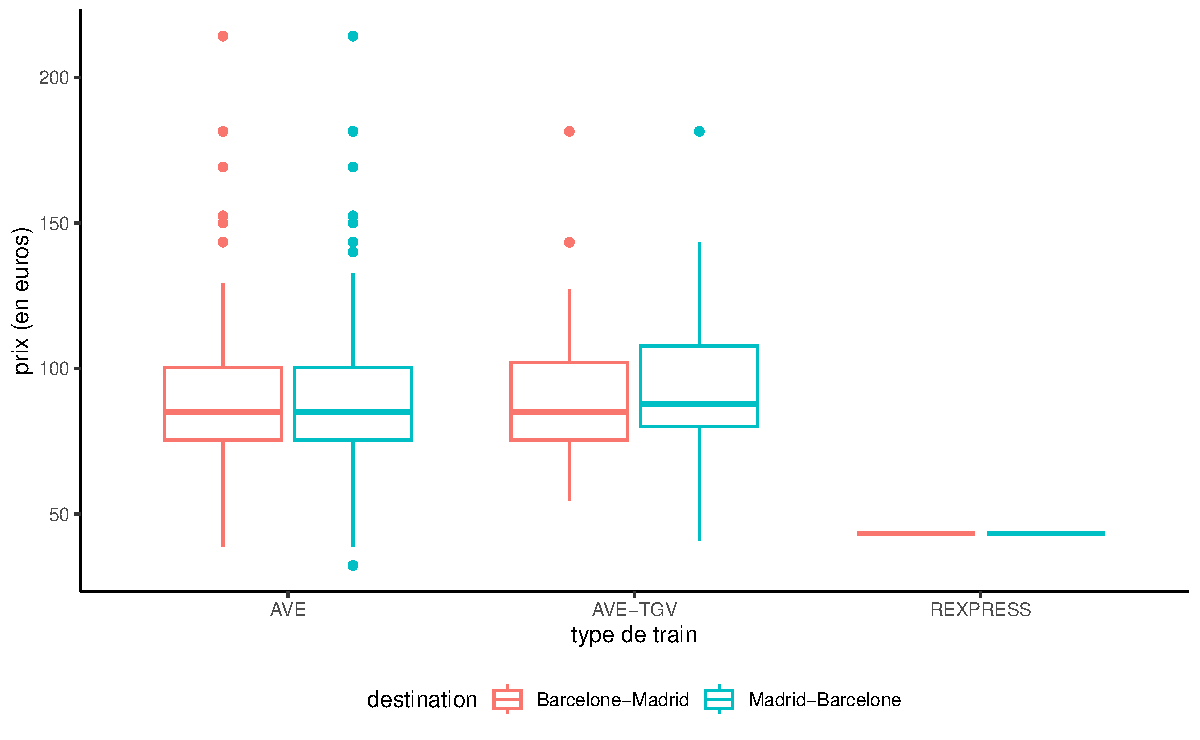
\includegraphics[width=1\textwidth,height=\textheight]{./01-analyseexploratoire_files/figure-pdf/fig-renfe-aed4-1.pdf}

}

\caption{\label{fig-renfe-aed4}Boîte à moustaches du prix de billets de
train de Renfe en fonction de la destination et du type de train.}

\end{figure}

On pourrait soupçonner que les trains étiquetés \texttt{AVE} sont plus
rapides, sachant que c'est l'acronyme de \emph{Alta Velocidad Española},
littéralement haute vitesse espagnole. Qu'en est-il des distinctions
entre les deux types de trains étiquetés AVE? Selon
\href{https://www.renfe-sncf.com/rw-en/services/a-unique-experience/Pages/services.aspx}{le
site de la SNCF}, les trains AVE-TGV sont des partenariats entre la
Renfe et la SNCF et effectuent des liaisons entre la France et
l'Espagne.

Les prix sont beaucoup plus élevés, en moyenne plus de deux fois plus
que les trains régionaux. Les écarts de prix importants (l'écart type
est de 20 euros) indique qu'il y a peut-être d'autres sources
d'hétérogénéité, mais on pourrait soupçonner que la Renfe pratique la
tarification dynamique. Il y un seul temps de parcours prévu pour les
trains AVE-TGV. On ne note pas de différence de prix notable selon la
direction ou le type de train grande vitesse, mais peut-être que les
tarifs ou la classe disponibles diffèrent selon que le train ou non est
en partenariat avec la compagnie française.

On n'a pas encore considéré le tarif et la classe des billets, hormis
pour les trains RegioExpress. On voit dans la
Figure~\ref{fig-renfe-aed7} une forte différente dans l'hétérogénéité
des prix selon le tarif; le tarif Promo prend plusieurs valeurs
distinctes, tandis que les tarifs AdultoIda et Flexible semblent ne
prendre que quelques valeurs. La première classe (\texttt{Preferente})
est plus chère et il y a moins d'observations dans ce groupe. La classe
Turista est la classe la moins dispendieuse et la plus populaire.
\href{http://web.archive.org/web/20161111134241/http://www.renfe.com/viajeros/tarifas/billete_promo.html}{\texttt{TuristaPlus}}
offre plus de confort, tandis que \texttt{TuristaSolo} permet d'obtenir
un siège individuel.

Côté tarif,
\href{http://web.archive.org/web/20161111134241/http://www.renfe.com/viajeros/tarifas/billete_promo.html}{Promo}
et
\href{http://web.archive.org/web/20161110220249/http://www.renfe.com/viajeros/tarifas/billete_promoplus.html}{PromoPlus}
permette d'obtenir des rabais pouvant aller jusqu'à respectivement 70\%
et 65\%. Les annulations et changements ne sont pas possibles avec
Promo, mais disponibles avec PromoPlus moyennant une pénalité équivalent
à 30-20\% du prix du billet. Le tarif
\href{http://web.archive.org/web/20161108192609/http://www.renfe.com/viajeros/tarifas/billete_flexible.html}{Flexible}
est disponible au même prix que les billets réguliers, avec des
bénéfices additionnels.

\begin{Shaded}
\begin{Highlighting}[]
\NormalTok{renfe }\SpecialCharTok{|\textgreater{}} 
  \FunctionTok{subset}\NormalTok{(tarif  }\SpecialCharTok{!=} \StringTok{"AdultoIda"}\NormalTok{) }\SpecialCharTok{|\textgreater{}}
  \FunctionTok{ggplot}\NormalTok{(}\FunctionTok{aes}\NormalTok{(}\AttributeTok{y =}\NormalTok{ prix, }
             \AttributeTok{x =}\NormalTok{ classe, }
             \AttributeTok{col =}\NormalTok{ tarif)) }\SpecialCharTok{+} 
    \FunctionTok{geom\_boxplot}\NormalTok{() }\SpecialCharTok{+} 
    \FunctionTok{labs}\NormalTok{(}\AttributeTok{y =} \StringTok{"prix (en euros)"}\NormalTok{,}
         \AttributeTok{x =} \StringTok{"classe"}\NormalTok{,}
         \AttributeTok{color =} \StringTok{"tarif"}\NormalTok{) }\SpecialCharTok{+}
    \FunctionTok{theme}\NormalTok{(}\AttributeTok{legend.position =} \StringTok{"bottom"}\NormalTok{)}
\end{Highlighting}
\end{Shaded}

\begin{figure}[ht!]

{\centering 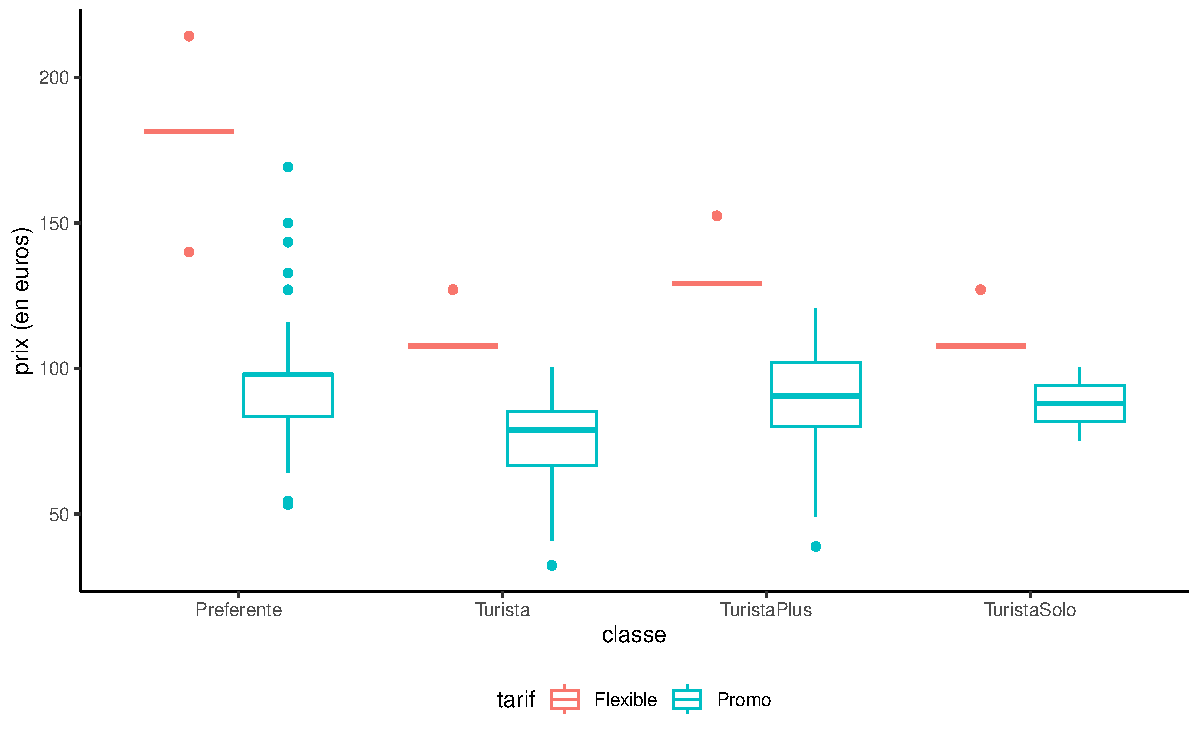
\includegraphics[width=1\textwidth,height=\textheight]{./01-analyseexploratoire_files/figure-pdf/fig-renfe-aed6-1.pdf}

}

\caption{\label{fig-renfe-aed6}Boîte à moustaches du prix en fonction du
tarif et de la classe de billets de trains à haute vitesse de la Renfe.}

\end{figure}

\begin{Shaded}
\begin{Highlighting}[]
\FunctionTok{ggplot}\NormalTok{(}\AttributeTok{data =}\NormalTok{ renfe, }
       \AttributeTok{mapping =} \FunctionTok{aes}\NormalTok{(}\AttributeTok{x =}\NormalTok{ prix, }
                     \AttributeTok{y=}\NormalTok{..density.., }
                     \AttributeTok{fill =}\NormalTok{ tarif)) }\SpecialCharTok{+}
    \FunctionTok{geom\_histogram}\NormalTok{(}\AttributeTok{binwidth =} \DecValTok{5}\NormalTok{) }\SpecialCharTok{+}
    \FunctionTok{labs}\NormalTok{(}\AttributeTok{x =} \StringTok{"prix (en euros)"}\NormalTok{, }
         \AttributeTok{y =} \StringTok{"densité"}\NormalTok{) }\SpecialCharTok{+} 
    \FunctionTok{theme}\NormalTok{(}\AttributeTok{legend.position =} \StringTok{"bottom"}\NormalTok{)}
\end{Highlighting}
\end{Shaded}

\begin{figure}[ht!]

{\centering 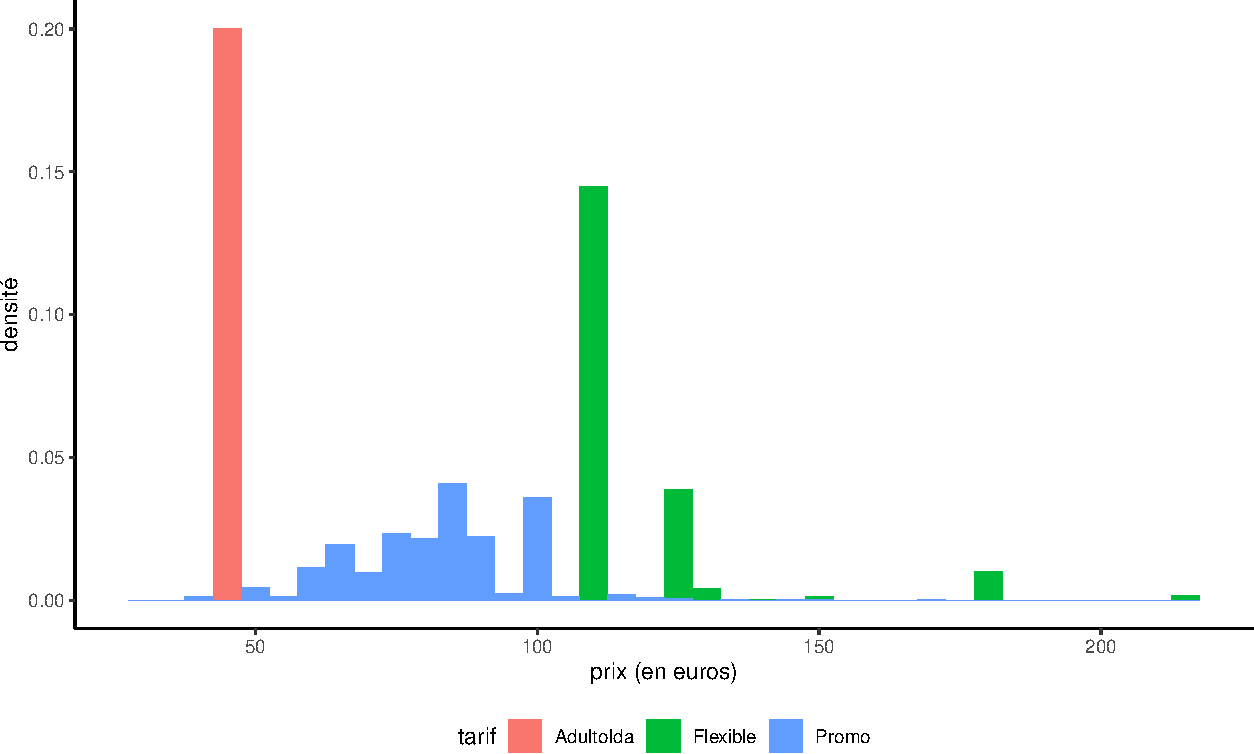
\includegraphics[width=1\textwidth,height=\textheight]{./01-analyseexploratoire_files/figure-pdf/fig-renfe-aed7-1.pdf}

}

\caption{\label{fig-renfe-aed7}Histogrammes du prix en fonction du tarif
de billets de trains de la Renfe.}

\end{figure}

\begin{Shaded}
\begin{Highlighting}[]
\NormalTok{renfe }\SpecialCharTok{|\textgreater{}}
\NormalTok{  dplyr}\SpecialCharTok{::}\FunctionTok{subset}\NormalTok{(tarif  }\SpecialCharTok{==} \StringTok{"Flexible"}\NormalTok{) }\SpecialCharTok{|\textgreater{}}
\NormalTok{  dplyr}\SpecialCharTok{::}\FunctionTok{count}\NormalTok{(prix, classe)}
\end{Highlighting}
\end{Shaded}

\hypertarget{tbl-renfeaedrep}{}
\begin{table}
\caption{\label{tbl-renfeaedrep}Nombre de billets au tarif Flexible selon le prix de vente. }

\centering
\begin{tabular}[t]{rlr}
\toprule
prix & classe & n\\
\midrule
107.7 & Turista & 1050\\
107.7 & TuristaSolo & 67\\
127.1 & Turista & 285\\
127.1 & TuristaSolo & 9\\
129.3 & TuristaPlus & 31\\
\addlinespace
140.0 & Preferente & 2\\
152.5 & TuristaPlus & 10\\
181.5 & Preferente & 78\\
214.2 & Preferente & 12\\
\bottomrule
\end{tabular}
\end{table}

On note que la répartition des prix pour les billets de classe Flexible
est inhabituelle. Notre boîte à moustaches est écrasée et l'écart
interquartile semble nul, même si quelques valeurs inexpliquées sont
aussi présentes. L'écrasante majorité des billets Flexibles sont en
classe Turista, donc ça pourrait être dû à un (trop) faible nombre de
billets dans chaque catégorie. On peut rejeter cette hypothèse en
calculant le nombre de trains au tarif Flexible pour les différents
types de billets, comme dans le Tableau~\ref{tbl-renfeaedrep}. Ni la
durée, ni le type de train, ni la destination n'expliquent pas pourquoi
le prix de certains billets Flexibles est plus faible ou élevés. Le prix
des billets Promo est plus faible, et les billets au tarif Preferente
(la première classe) sont plus élevés.

On peut résumer notre brève analyse exploratoire:

\begin{itemize}
\tightlist
\item
  plus de 91\% des trains sont des trains à grande vitesse AVE.
\item
  le temps de trajet dépend du type de train: les trains à grande
  vitesse mettent 3h20 au maximum pour relier Madrid et Barcelone.
\item
  les temps de trajets sont ceux annoncés (variable discrète avec 17
  valeurs uniques, dont 13 pour les trains AVE)
\item
  le prix de trains RegioExpress est fixe (43.25€); tous ces billets
  sont dans la classe Turista et au tarif Adulto Ida. 57\% de ces trains
  vont de Barcelone à Madrid. La durée du trajet pour les RegioExpress
  est de 9h22 de Barcelona à Madrid, 18 minutes de plus que dans l'autre
  direction.
\item
  les billets en classe\texttt{Preferente} sont plus chers et moins
  fréquents. La classe \texttt{Turista} est la classe la moins
  dispendieuse et la plus populaire. \texttt{TuristaPlus} offre plus de
  confort, tandis que \texttt{TuristaSolo} permet d'obtenir un siège
  individuel.
\item
  selon le
  \href{https://www.renfe.com/es/es/viajar/tarifas/billetes.html}{site
  web de la Renfe}, les billets au tarif \texttt{Flexible} « viennent
  avec des offres additionnelles qui permettent au passagers d'échanger
  leurs billets ou annuler s'ils manquent leurs trains. »; en
  contrepartie, ces billets sont plus chers et leur tarif est fixe sauf
  une poignée de billets dont le prix reste inexpliqué.
\item
  la distribution des prix des billets de TGV au tarif \texttt{Promo}
  est plus ou moins symmétrique, tandis que les billets au tarif
  \texttt{Flexible} apparaissent tronqués à gauche (le prix minimum pour
  ces billets est 107.7€ dans l'échantillon).
\item
  la Renfe pratique la tarification dynamique pour les billets au tarif
  promotionnel \texttt{Promo}: ces derniers peuvent être jusqu'à 70\%
  moins chers que les billets à prix régulier lorsqu'achetés via
  l'agence officielle ou le site de Renfe. Ces billets ne peuvent être
  ni remboursés, ni échangés.
\item
  il n'y a pas d'indication à effet de quoi les prix varient selon la
  direction du trajet.
\end{itemize}

\hypertarget{commentaire-sur-les-graphiques}{%
\subsection{Commentaire sur les
graphiques}\label{commentaire-sur-les-graphiques}}

Si vous incluez un graphique (ou un tableau), il est important d'ajouter
une légende qui décrit le graphique et le résume, les noms de variables
(avec les unités) sur les axes, mais aussi de soigner le rendu et le
formatage pour obtenir un produit fini propre, lisible et cohérent: en
particulier, votre description devrait coïncider avec le rendu. Votre
graphique raconte une histoire, aussi prenez-soin que cette dernière
soit nécessaire et attrayante.

\begin{tcolorbox}[standard jigsaw,title=\textcolor{quarto-callout-note-color}{\faInfo}\hspace{0.5em}{En résumé}, colbacktitle=quarto-callout-note-color!10!white, bottomrule=.15mm, toptitle=1mm, toprule=.15mm, opacitybacktitle=0.6, bottomtitle=1mm, titlerule=0mm, rightrule=.15mm, colback=white, arc=.35mm, leftrule=.75mm, left=2mm, coltitle=black, colframe=quarto-callout-note-color-frame, opacityback=0]

\begin{itemize}
\tightlist
\item
  Une base de données est normalement constituée de plusieurs variables
  (colonnes); les lignes représentent les différentes observations.
\item
  On classifie grossièrement les variables en variables catégorielles
  (nominales, ordinales ou binaires) et numériques (continues,
  entières).
\item
  L'analyse exploratoire est une procédure dynamique qui sert à mieux
  comprendre les données pour proposer des modèles adéquats. Elle
  consiste à poser des questions et à raffiner les conclusions à l'aide
  de tableaux résumés et de graphique.
\item
  Le nettoyage et la validation des données est la première étape de
  toute analyse. On peut déclarer nos attentes et l'utiliser pour
  vérifier de la conformité de notre base de données (en utilisant des
  outils comme le
  \href{https://github.com/rich-iannone/pointblank}{paquet
  \texttt{pointblank}}.
\item
  Une bonne compréhension des données est nécessaire avant d'envisager
  la modélisation.
\item
  Il faut déclarer correctement les variables explicatives catégorielles
  (souvent encodées avec des entiers).
\item
  L'utilisation de graphiques est privilégiée par rapport aux tableaux:
  une image vaut mille mots.
\item
  Les graphiques usuels employés sont l'histogramme et la
  boîte-à-moustaches (données numériques) et le diagramme à bande
  (données catégorielles). L'utilisation de diagramme circulaires est à
  proscrire.
\item
  On peut utiliser les couleurs ou la forme pour ajouter une dimension.
\item
  Toujours utiliser une palette de couleurs pour daltoniens.
\item
  Un graphique devrait toujours inclure une légende globale décrivant la
  représentation (en plus d'être discuté dans le texte), une légende
  pour les axes et des unités. Les caractères doivent être lisibles
  (suffisamment grands).
\item
  Une analyse exploratoire inclut un résumé des principales trouvailles.
\end{itemize}

\end{tcolorbox}

\hypertarget{analyse-factorielle}{%
\chapter{Réduction de la dimension}\label{analyse-factorielle}}

\hypertarget{introduction-1}{%
\section{Introduction}\label{introduction-1}}

Ce chapitre traite de réduction de la dimensionalité d'un problème
d'analyse multidimensionnelle. On dispose de \(p\) variables
\(X_1, \ldots, X_p\): comment résumer cet ensemble avec moins de
variables (disons \(k\)) tout en conservant le plus de variabilité
possible? Nous couvrons deux méthodes dans ce chapitre: la première,
intitulée \textbf{analyse en composantes principales}, cherche à
\textbf{réduire le nombre de variables explicatives} tout en préservant
le plus possible de variabilité exprimée et en créant de nouvelles
variables explicatives qui ne sont pas corrélées les unes avec les
autres.

La deuxième, appelée analyse factorielle exploratoire, cherche à
expliquer la structure de corrélation entre les \(p\) variables à l'aide
d'un nombre restreint de facteurs. Elle répond aux questions suivantes:

\begin{itemize}
\tightlist
\item
  Y a-t-il des groupements de variables?
\item
  Est-ce que les variables faisant partie d'un groupement semblent
  mesurer certains aspects d'un facteur commun (non observé)?
\end{itemize}

De tels groupements peuvent être détecté si plusieurs variables sont
très corrélées entre elles. Une analyse factorielle cherchera à
identifier automatiquement ces groupes de variables.

Les facteurs sont des variables latentes qui mesurent des constructions.
Par exemple, l'habileté quantitative, habileté sociale, importance
accordée à la qualité du service, importance accordée à la loyauté,
habileté de leader, etc.

L'analyse factorielle est aussi une méthode de réduction du nombre de
variables. En effet, une fois qu'on a identifié les facteurs, on peut
remplacer les variables individuelles par un résumé pour chaque facteur
(qui est souvent la moyenne des variables qui font partie du facteur).

\hypertarget{coefficient-de-corruxe9lation-linuxe9aire}{%
\section{Coefficient de corrélation
linéaire}\label{coefficient-de-corruxe9lation-linuxe9aire}}

On veut examiner la relation entre deux variables \(X_j\) et \(X_k\) et
on dispose de \(n\) couples d'observations, où \(x_{i, j}\)
(respectivement \(x_{i, k}\)) est la valeur de la variable \(X_j\)
(\(X_k\)) pour la \(i\)e observation.

Le coefficient de corrélation linéaire entre \(X_j\) et \(X_k\), que
l'on note \(r_{j, k}\), cherche à mesurer la force de la relation
linéaire entre deux variables, c'est-à-dire à quantifier à quel point
les observations sont alignées autour d'une droite. Le coefficient de
corrélation est \begin{align*}
r_{j, k} &= \frac{\widehat{\mathsf{Co}}(X_j, X_k)}{\{\widehat{\mathsf{Va}}(X_j) \widehat{\mathsf{Va}}(X_k)\}^{1/2}} 
%\\&=\frac{\sum_{i=1}^n (x_{i, j}-\overline{x}_j)(x_{i, k} -\overline{x}_{k})}{\left\{\sum_{i=1}^n (x_{i, j}-\overline{x}_j)^2 \sum_{i=1}^n(x_{i, k} -\overline{x}_{k})^2\right\}^{1/2}}
\end{align*}

Les propriétés les plus importantes du coefficient de corrélation
linéaire \(r\) sont les suivantes:

\begin{enumerate}
\def\labelenumi{\arabic{enumi})}
\tightlist
\item
  \(-1 \leq r \leq 1\);
\item
  \(r=1\) (respectivement \(r=-1\)) si et seulement si les \(n\)
  observations sont exactement alignées sur une droite de pente positive
  (négative). C'est-à-dire, s'il existe deux constantes \(a\) et \(b>0\)
  (\(b<0\)) telles que \(y_i=a+b x_i\) pour tout \(i=1, \ldots, n\).
\end{enumerate}

Règle générale,

\begin{itemize}
\tightlist
\item
  Le signe de la corrélation détermine l'orientation de la pente
  (négative ou positive)
\item
  Plus la corrélation est près de 1 en valeur absolue, plus les points
  auront tendance à être alignés autour d'une droite.
\item
  Lorsque la corrélation est presque nulle, les points n'auront pas
  tendance à être alignés autour d'une droite. Il est très important de
  noter que cela n'implique pas qu'il n'y a pas de relation entre les
  deux variables. Cela implique seulement qu'il n'y a pas de
  \textbf{relation linéaire} entre les deux variables. La
  Figure~\ref{fig-datasaurus} montre bien ce point: ces jeux de données
  ont la même corrélation linéaire (quasi-nulle), mais ne sont pas
  clairement pas indépendantes puisqu'elles permettent de dessiner un
  dinosaure ou une étoile.
\end{itemize}

\begin{figure}[ht!]

{\centering 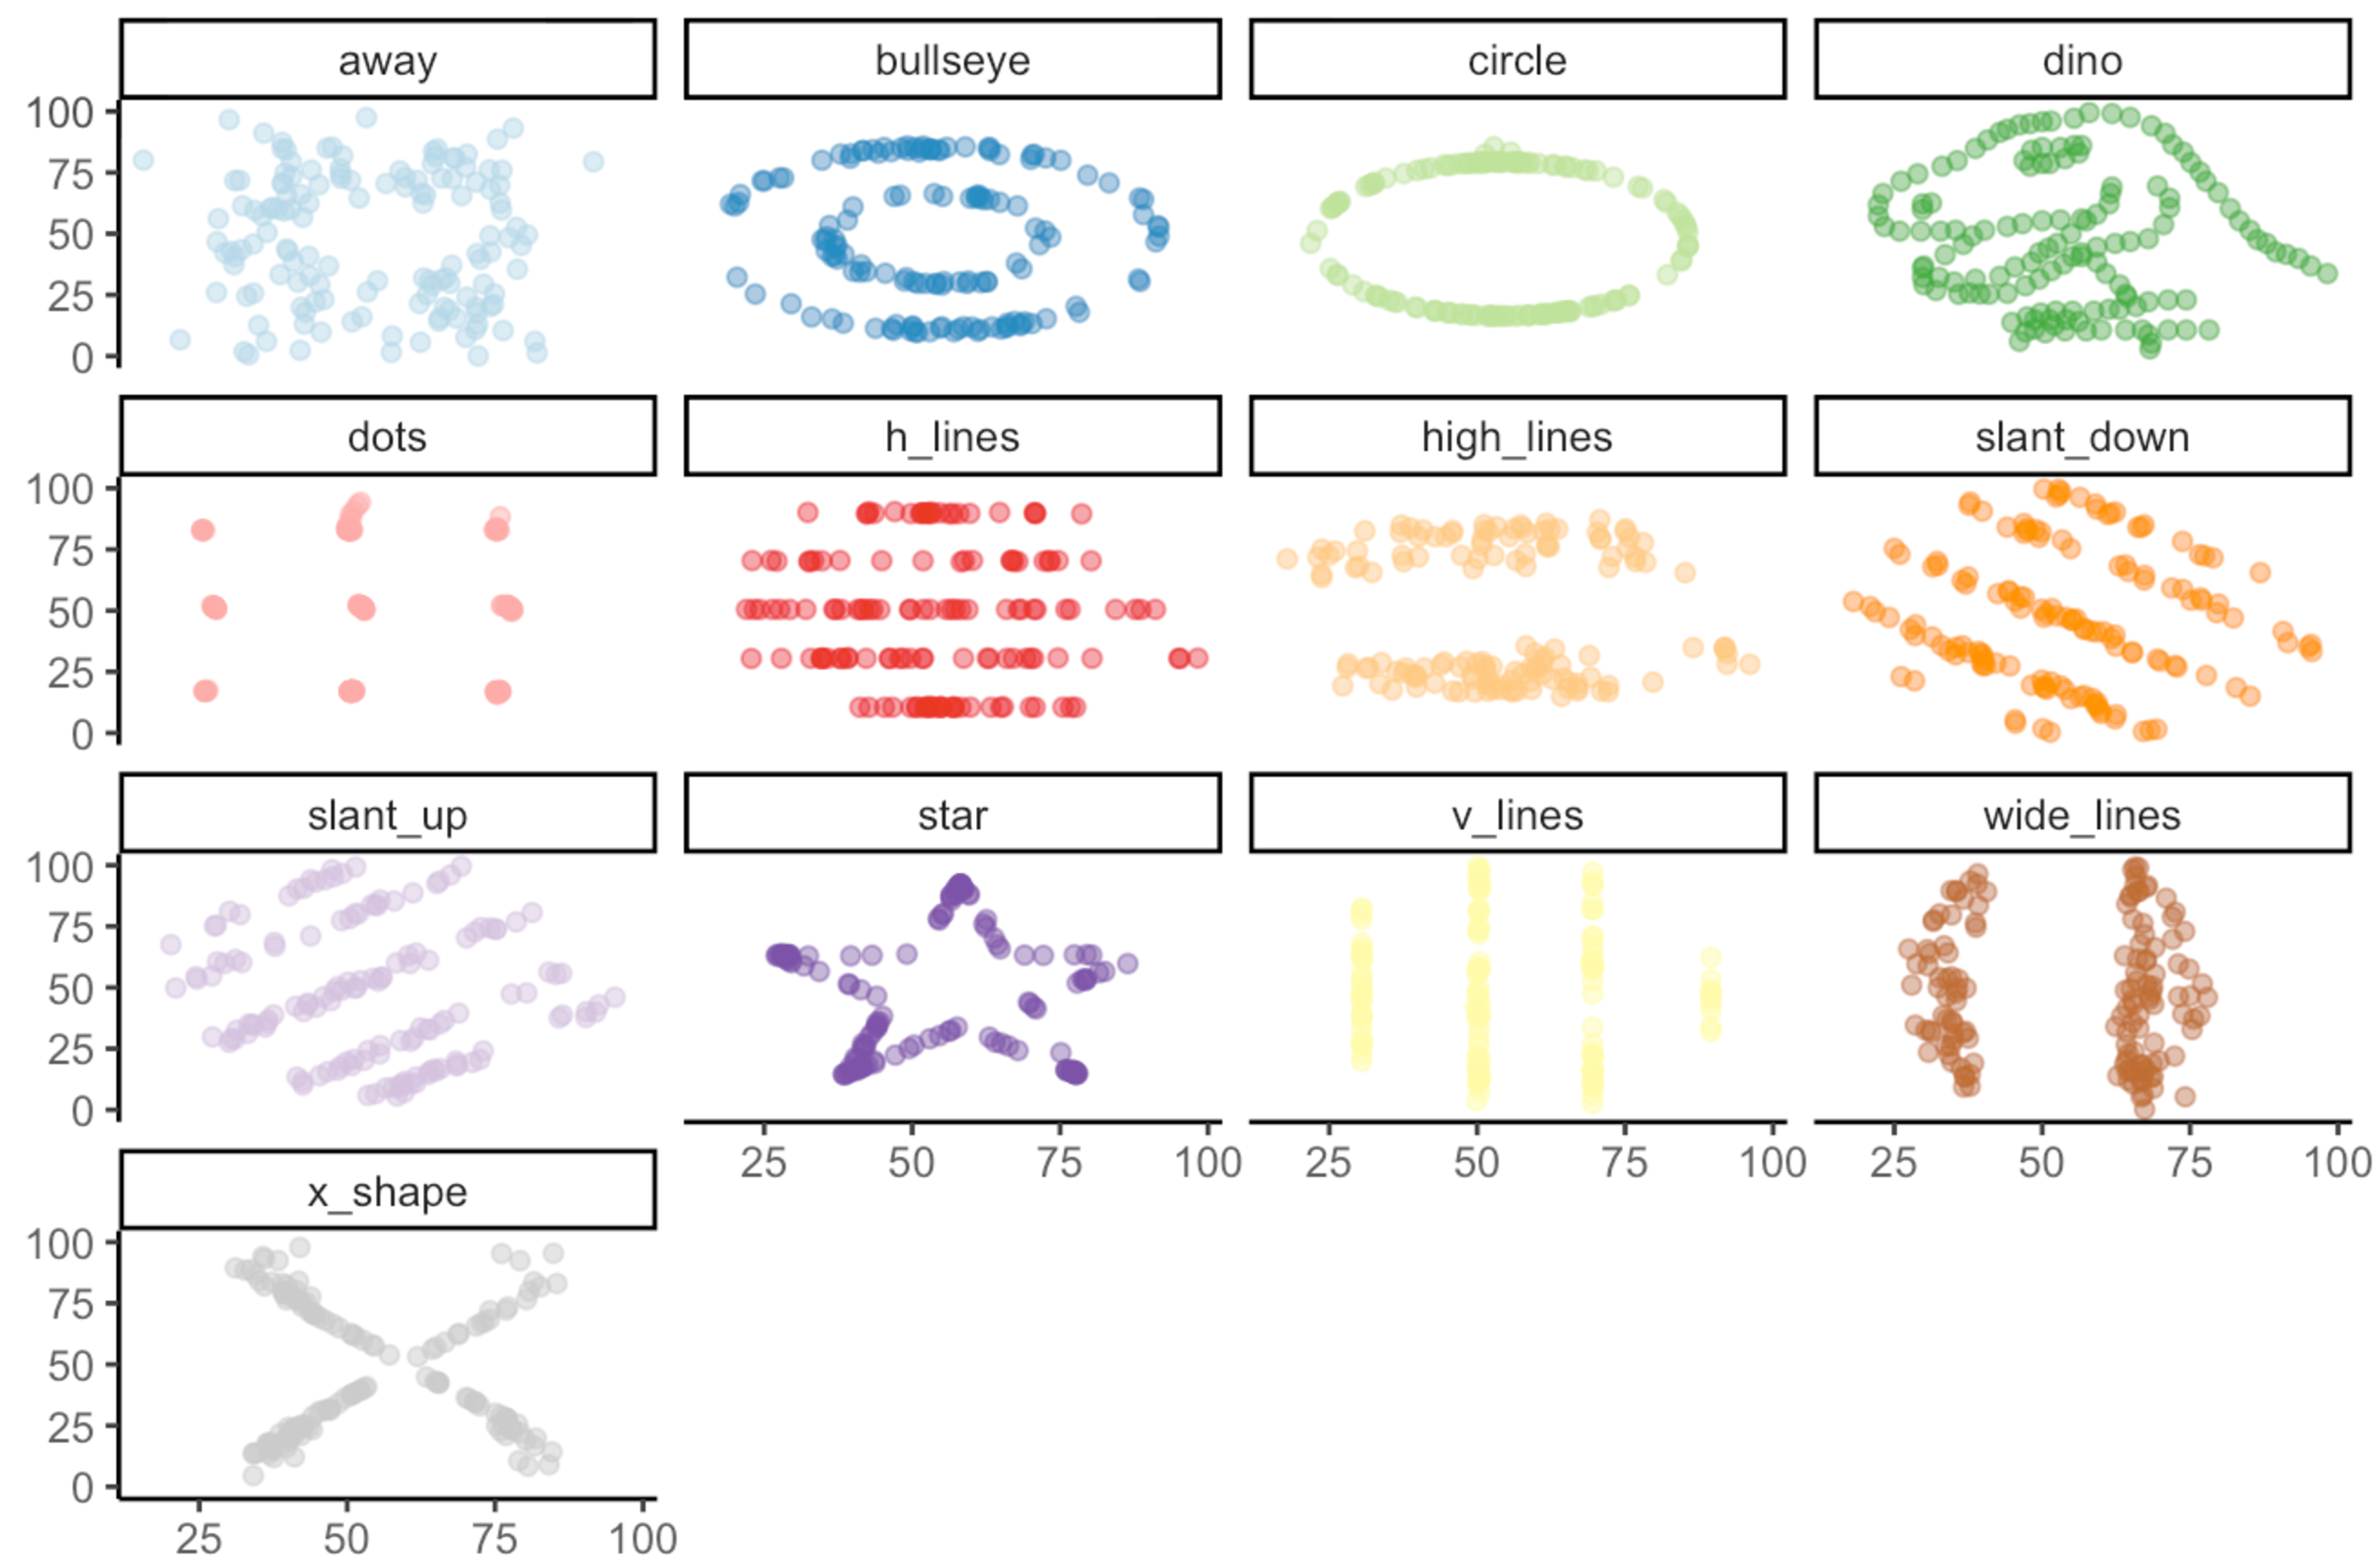
\includegraphics{./figures/DataSaurusDozen.pdf}

}

\caption{\label{fig-datasaurus}Datasaurus (Alberto Cairo): une douzaine
de jeux de données qui ont les mêmes statistiques descriptives (à deux
décimales près) et une faible corrélation, mais qui sont visuellement
distincts.}

\end{figure}

La matrice de corrélation entre \(X_1, \ldots, X_p\), dont l'entrée
\((i, j)\) contient la corrélation entre \(X_i\) et \(X_j\), est une
matrice symmétrique dont les éléments de la diagonale sont égaux à 1. À
mesure que le nombre de variables augmente, le nombre de corrélations à
estimer augmente: puisque la matrice est \(p \times p\), ce nombre
augmente comme le carré du nombre de variables explicatives.
L'estimation ne sera pas fiable à moins que \(n \gg p\).

\hypertarget{pruxe9sentation-des-donnuxe9es}{%
\section{Présentation des
données}\label{pruxe9sentation-des-donnuxe9es}}

Le questionnaire suivant porte sur une étude dans un magasin. Pour les
besoins d'une enquête, on a demandé à 200 consommateurs adultes de
répondre aux questions suivantes par rapport à un certain type de
magasin sur une échelle de 1 à 5, où

\begin{enumerate}
\def\labelenumi{\arabic{enumi}.}
\tightlist
\item
  pas important
\item
  peu important
\item
  moyennement important
\item
  assez important
\item
  très important
\end{enumerate}

Pour vous, à quel point est-ce important\ldots

\begin{enumerate}
\def\labelenumi{\arabic{enumi}.}
\tightlist
\item
  que le magasin offre de bons prix tous les jours?
\item
  que le magasin accepte les cartes de crédit majeures (Visa,
  Mastercard)?
\item
  que le magasin offre des produits de qualité?
\item
  que les vendeurs connaissent bien les produits?
\item
  qu'il y ait des ventes spéciales régulièrement?
\item
  que les marques connues soient disponibles?
\item
  que le magasin ait sa propre carte de crédit?
\item
  que le service soit rapide?
\item
  qu'il y ait une vaste sélection de produits?
\item
  que le magasin accepte le paiement par carte de débit?
\item
  que le personnel soit courtois?
\item
  que le magasin ait en stock les produits annoncés?
\end{enumerate}

Les statistiques descriptives ainsi que la matrice des corrélations sont
obtenues en exécutant les lignes suivantes:

\begin{Shaded}
\begin{Highlighting}[]
\FunctionTok{data}\NormalTok{(factor, }\AttributeTok{package =} \StringTok{"hecmulti"}\NormalTok{)}
\CommentTok{\# Matrice de corrélation}
\FunctionTok{cor}\NormalTok{(factor)}
\CommentTok{\# Statistiques descriptives}
\FunctionTok{summary}\NormalTok{(factor)}
\end{Highlighting}
\end{Shaded}

\hypertarget{tbl-corrmat}{}
\begin{table}
\caption{\label{tbl-corrmat}Matrice de corrélation de factor. }

\centering
\begin{tabular}{lrrrrrrrrrrrr}
\toprule
  & x1 & x2 & x3 & x4 & x5 & x6 & x7 & x8 & x9 & x10 & x11 & x12\\
\midrule
x1 &  & -0.08 & -0.14 & -0.07 & 0.38 & -0.01 & -0.10 & -0.13 & -0.03 & -0.11 & -0.12 & -0.01\\
x2 &  &  & 0.04 & -0.02 & -0.08 & 0.06 & 0.50 & 0.01 & -0.01 & 0.43 & -0.12 & 0.07\\
x3 &  &  &  & 0.10 & -0.06 & 0.39 & 0.00 & 0.05 & 0.47 & 0.08 & 0.13 & 0.46\\
x4 &  &  &  &  & -0.05 & 0.06 & 0.08 & 0.57 & 0.01 & 0.09 & 0.50 & 0.09\\
x5 &  &  &  &  &  & -0.04 & -0.04 & -0.02 & 0.03 & -0.07 & -0.06 & -0.07\\
\addlinespace
x6 &  &  &  &  &  &  & 0.07 & 0.04 & 0.32 & 0.07 & -0.04 & 0.32\\
x7 &  &  &  &  &  &  &  & 0.09 & -0.02 & 0.51 & -0.03 & 0.02\\
x8 &  &  &  &  &  &  &  &  & -0.03 & 0.16 & 0.55 & 0.04\\
x9 &  &  &  &  &  &  &  &  &  & 0.01 & 0.02 & 0.39\\
x10 &  &  &  &  &  &  &  &  &  &  & 0.01 & 0.02\\
\addlinespace
x11 &  &  &  &  &  &  &  &  &  &  &  & 0.05\\
x12 &  &  &  &  &  &  &  &  &  &  &  & \\
\bottomrule
\end{tabular}
\end{table}

\begin{figure}[ht!]

{\centering 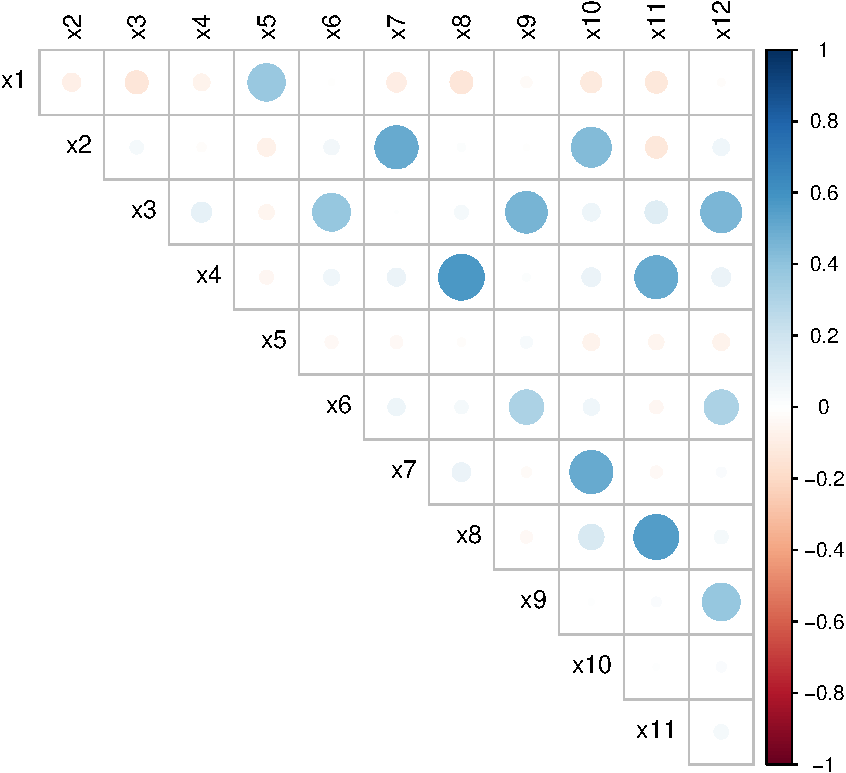
\includegraphics[width=1\textwidth,height=\textheight]{./02-analysefactorielle_files/figure-pdf/fig-corrmat-1.pdf}

}

\caption{\label{fig-corrmat}Corrélogramme de la base de données
\texttt{factor}.}

\end{figure}

\begin{table}

\caption{\label{tbl-statdescriptfactor}\textbf{?(caption)}}\begin{minipage}[t]{\linewidth}
\subcaption{\label{tbl-statdescriptfactor-1}}

{\centering 

\begin{tabu} to \linewidth {>{\raggedleft}X>{\raggedleft}X>{\raggedleft}X>{\raggedleft}X}
\toprule
moyenne & écart-type & min & max\\
\midrule
2.26 & 1.13 & 1 & 5\\
2.51 & 1.24 & 1 & 5\\
3.00 & 1.19 & 1 & 5\\
2.91 & 1.33 & 1 & 5\\
3.55 & 1.17 & 1 & 5\\
\addlinespace
2.14 & 1.14 & 1 & 5\\
1.82 & 1.06 & 1 & 5\\
2.92 & 1.32 & 1 & 5\\
3.04 & 1.12 & 1 & 5\\
2.59 & 1.32 & 1 & 5\\
\addlinespace
2.98 & 1.33 & 1 & 5\\
3.45 & 1.16 & 1 & 5\\
\bottomrule
\end{tabu}

}

\end{minipage}%

\end{table}

On voit dans la Figure~\ref{fig-corrmat} que quelques groupes de
variables sont corrélés entre eux. On peut également regrouper certaines
questions sous des thèmes manuellement: le but de l'analyse factorielle
sera d'automatiser ce regroupement.

\hypertarget{analyse-en-composantes-principales}{%
\section{Analyse en composantes
principales}\label{analyse-en-composantes-principales}}

Le but de l'analyse en composantes principales est de réduire le nombre
de variables explicatives. En partant de \(p\) variables
\(X_1, \ldots, X_p\), on forme de nouvelles variables qui sont des
combinaisons linéaires des variables originales, \begin{align*}
C_j &= w_{j1} X_1 + w_{j2} X_2 + \cdots + w_{jp} X_p, \qquad (j=1, \ldots, p),
\end{align*} de telle sorte que

\begin{itemize}
\tightlist
\item
  La première variable formée, \(C_1\), appelée première composante
  principale, possède la variance maximale parmi toutes les combinaisons
  linéaires sous la contrainte
  \(w_{11}^2 + \cdots + w_{1p}^2=1\)\footnote{Les contraintes sont
    nécessaires afin de standardiser le problème car il serait possible
    d'avoir des variances infinies sinon.}.
\item
  Pour \(j=2, \ldots, p\), la \(j\)e composante principale \(C_j\)
  possède la variance maximale parmi toutes les combinaisons linéaires
  qui sont non corrélées avec \(C_1, \ldots, C_{j-1}\) sous la
  contrainte \(w_{j1}^2 + \cdots + w_{jp}^2=1\).
\end{itemize}

Ainsi, les composantes principales forment un ensemble de variables non
corrélées entre elles, qui récupèrent en ordre décroissant le plus
possible de la variance des variables originales. La somme des variances
des \(p\) composantes principales est égale à la somme des variances des
\(p\) variables originales.

Mathématiquement, les composantes principales correspondent aux vecteurs
propres de la matrice de covariance, mais on peut également utiliser la
matrice de corrélation\footnote{La fonction \texttt{princomp} peut
  directement utiliser la base de données numériques, ou la matrice de
  covariance. Dans le premier cas, on peut spécifier que l'on veut la
  décomposition de la matrice de corrélation à l'aide de l'argument,
  \texttt{cor}}. L'avantage de la matrice de corrélation (ou de la
standardisation des variables) est que l'unité de mesure n'impacte pas
le résultat; autrement, un poids plus important est attribué aux
variables qui ont la plus forte hétérogénéité.

Si on conserve toutes les composantes principales, cela revient à
changer le système de coordonnées dans lequel sont exprimées nos
observations en effectuant une rotation: avec deux variables, on on
trouve la direction dans le système 2D dans lequel l'étendue est la plus
grande. Si une simple rotation peut sembler inutile, la méthode est fort
utile en haute dimension. On espère en général qu'un petit nombre de
composantes principales réussira à expliquer la plus grande partie de la
variance totale.

\begin{figure}[ht!]

{\centering 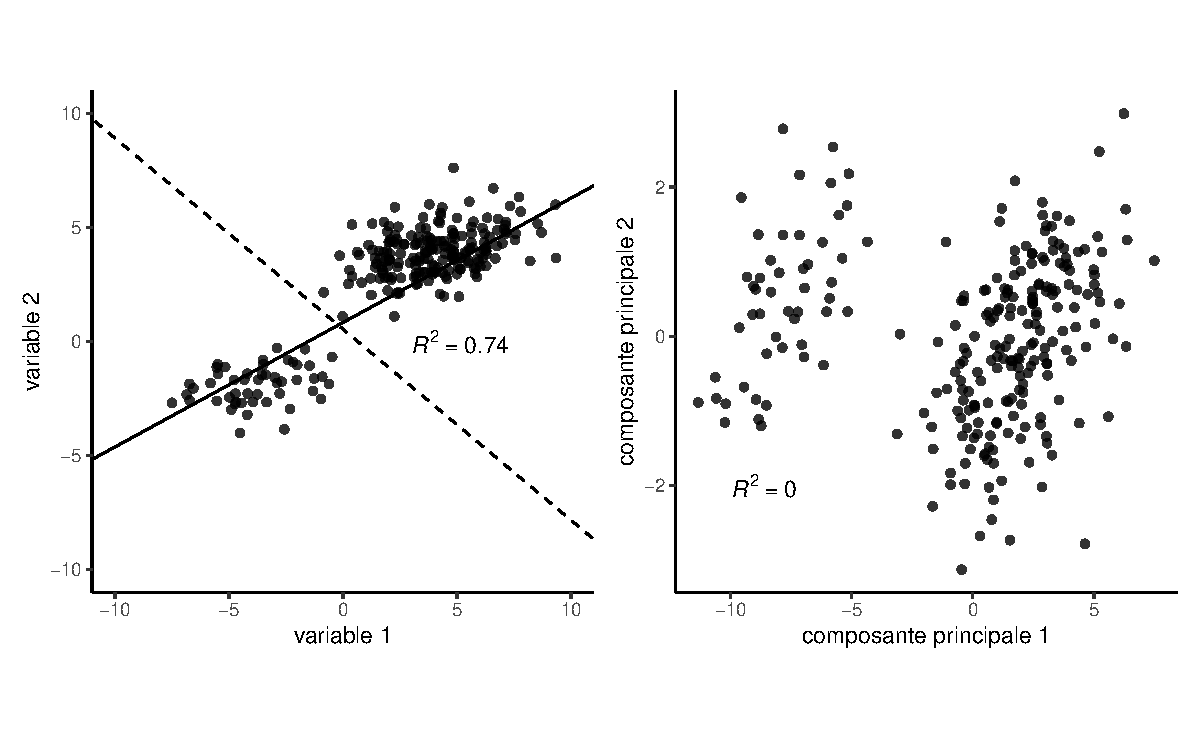
\includegraphics[width=0.9\textwidth,height=\textheight]{./02-analysefactorielle_files/figure-pdf/fig-acprotation-1.pdf}

}

\caption{\label{fig-acprotation}Nuage de points avant (gauche) et après
(droite) analyse en composantes principales. Les directions des
composantes principales (lignes pleines et traitillés), qui forment un
angle droit, sont ajoutées au nuage de points à gauche. On peut
constater que la corrélation entre les deux composantes principales est
nulle.}

\end{figure}

La figure Figure~\ref{fig-acprotation} démontre cette décomposition sur
des données bidimensionnelles simulées. La variance des données dans le
premier panneau est 13.51 pour l'axe des abscisse et 6.43 pour l'axe des
ordonnées avec une corrélation de 0.86, à comparer avec des variances de
18.65 et 1.21 et une corrélation nulle entre les deux composantes
principales.

Dans une analyse en composantes principales, on conservera un nombre
\(k<p\) de variables explicatives pour résumer les données. Ce outil est
utilisé à des fins exploratoires, puisqu'on n'implique pas de variable
réponse dans le modèle. L'analyse en composantes principales est utilisé
pour réduire la dimension afin de faire de la classification, de
l'analyse de regroupements et aussi réduire les coûts associés à ces
méthodes en projetant les données dans un sous-espace de dimension plus
faible.

En \textbf{R}, on effectue l'analyse en composantes principales avec la
fonction \texttt{princomp}\footnote{On pourrait aussi utiliser
  \texttt{eigen(cor(factor))} pour extraire directement la décomposition
  en valeurs propres/vecteurs propres, mais on n'aurait pas accès aux
  méthodes pour la visualisation.}.

La sortie contient

\begin{itemize}
\tightlist
\item
  l'écart-type de chaque composante, \texttt{acp\$sdev}
\item
  les poids \(w_{ij}\), appelés chargements (\emph{loadings}), qui
  donnent la correspondance entre le système de coordonnées des
  composantes principales et celui des variables \(\boldsymbol{X}\)
  originales.
\item
  les nouvelles coordonnées dans l'espace des composantes principales,
  \texttt{acp\$scores}
\end{itemize}

On peut représenter les données à l'aide d'un bigramme: c'est une nuage
de points de chaque observations dans l'espace des deux premières
composantes principales. Si on couple cela avec les directions offertes
par les chargements pour chacune des variables explicatives
\(X_1, \ldots, X_p\), il en ressort que certaines variables
augmentent/diminuent de pair. Ainsi, on voit dans
Figure~\ref{fig-biplot} que les variables \texttt{x3}, \texttt{x6},
\texttt{x9} et \texttt{x12} tendent dans la même direction, comme
\texttt{x4}, \texttt{x8} et \texttt{x11}. On reviendra sur ce point dans
une section subséquente.

Une fois qu'on a choisit le nombre de composantes, on pourrait ne
conserver que les \(k\) premières colonnes de la matrice des composantes
principales \texttt{acp\$scores} pour faire les graphiques ou pour
approximer la matrice de covariance. Il faut garder en tête qu'il faudra
néanmoins collecter les mêmes questions pour recréer les composantes
principales avec de nouvelles observations, ce qui est peu commode si ce
qu'on veut est réduire le coût de la collecte.

\begin{Shaded}
\begin{Highlighting}[]
\CommentTok{\# Analyse en composantes principales}
\CommentTok{\# de la matrice de corrélation}
\NormalTok{acp }\OtherTok{\textless{}{-}} \FunctionTok{princomp}\NormalTok{(factor, }\AttributeTok{cor =} \ConstantTok{TRUE}\NormalTok{)}
\FunctionTok{loadings}\NormalTok{(acp) }\CommentTok{\# chargements}
\FunctionTok{biplot}\NormalTok{(acp) }\CommentTok{\# bigramme}
\end{Highlighting}
\end{Shaded}

\begin{figure}[ht!]

{\centering 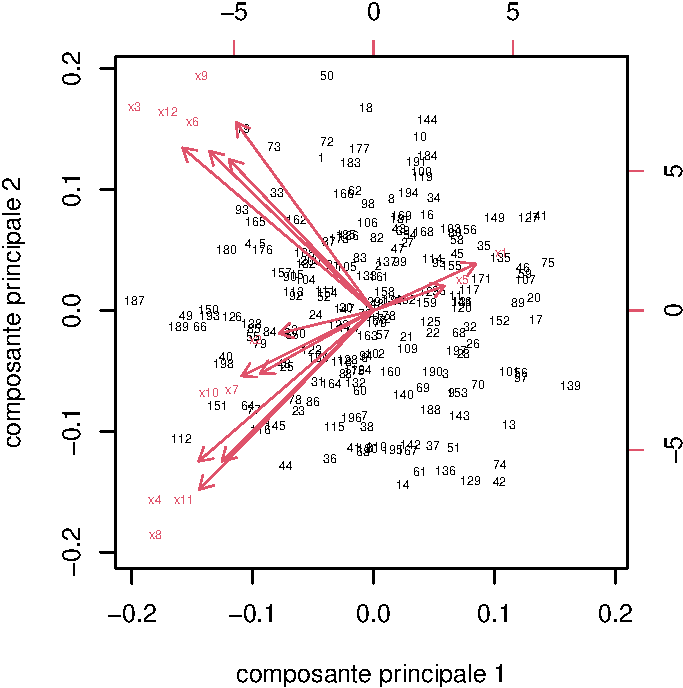
\includegraphics[width=1\textwidth,height=\textheight]{./02-analysefactorielle_files/figure-pdf/fig-biplot-1.pdf}

}

\caption{\label{fig-biplot}Bigramme: nuage de point des coordonnées des
deux premières composantes principales et direction selon chargements
des variables explicatives originales.}

\end{figure}

On peut étudier la sortie pour vérifier les propriétés de notre
décomposition. Le Tableau~\ref{tbl-eigenvalues} montre la variance de
chaque composante principale. Si on additionne l'ensemble des variances
(sans arrondir), on obtient une variance cumulative des 12 composantes
principales, 12, soit le même que le nombre de variables explicatives
puisque les variables standardisées ont variance unitaire. Si on calcule
la matrice de corrélation, \texttt{cor(acp\$scores)}, on remarquera que
la corrélation est nulle entre les variables.

\begin{table}

\caption{\label{tbl-eigenvalues}\textbf{?(caption)}}\begin{minipage}[t]{\linewidth}
\subcaption{\label{tbl-eigenvalues-1}}

{\centering 

\begin{tabu} to \linewidth {>{\centering}X>{\centering}X>{\centering}X>{\centering}X>{\centering}X>{\centering}X>{\centering}X>{\centering}X>{\centering}X>{\centering}X>{\centering}X>{\centering}X}
\toprule
C1 & C2 & C3 & C4 & C5 & C6 & C7 & C8 & C9 & C10 & C11 & C12\\
\midrule
2.43 & 2.00 & 1.94 & 1.30 & 0.74 & 0.69 & 0.57 & 0.54 & 0.51 & 0.47 & 0.46 & 0.36\\
\bottomrule
\end{tabu}

}

\end{minipage}%

\end{table}

\hypertarget{sec-acp-choix}{%
\subsection{Choix du nombre de composantes
principales}\label{sec-acp-choix}}

Si on désire réduire la dimension, il nous faudra choisir \(k \leq p\)
variables. Cette section traite du choix du nombre de variables
explicatives à retenir. Idéalement, ce nombre devrait être beaucoup plus
petit que le nombre original de variables.

Une première approche est de regarder le pourcentage de la variance
totale expliquée. Puisque les composantes principales sont ordonnées en
ordre décroissant de variance, on peut étudier la variance cumulative
des \(k\) premières composantes et choisir un nombre qui explique le
plus possible. Si l'ajout d'une variable augmente peu la variabilité
totale expliquée par l'ensemble, alors cette variable est probablement
superflue. On pourrait choisir un nombre de composantes pour expliquer
un pourcentage prédéfini de la vairance totale, disons 70\%. Deux autres
critères couramment employés sont:

\begin{itemize}
\tightlist
\item
  \textbf{critère du coude de Cattell}: ce critère consiste à
  sélectionner un nombre de composantes dans le diagramme d'éboulis
  (\texttt{screeplot}), un graphique des variances des composantes
  principales\footnote{Soit les valeurs propres de la matrice de
    covariance ou corrélation}. Habituellement, il y a une décroissance
  rapide de la variance suivie d'un plateau: on prendra le nombre de
  composantes qui correspond au \(k\) juste avant l'apparition du
  plateau (le début du coude, où il a stabilisation apparente). C'est un
  critère très subjectif, puisqu'il y a souvent plusieurs plateaux et
  que la variance peut décroître très lentement. On peut utiliser la
  fonction \texttt{screeplot} pour obtenir le diagramme d'éboulis mais
  il est facile de le créer manuellement et le résultat est
  esthétiquement plus réussi.
\item
  \textbf{critère de Kaiser}: un critère basé sur les valeurs propres de
  la matrice de corrélation. Le nombre de facteurs choisis est le nombre
  de composantes principales dont la variance est supérieures à 1.
  L'idée est de garder seulement les facteurs qui expliquent plus de
  variance qu'une variable individuelle.
\end{itemize}

Si on utilise le critère de Kaiser avec les données \texttt{factor}, on
conservera 4 composantes principales qui expliqueront 63.9 pourcent de
la variance totale des variables originales - voir le
Tableau~\ref{tbl-eigenvalues}. Le diagramme d'éboulis de la
Figure~\ref{fig-screeplot}, qui peut être produit avec la fonction
\texttt{hecmulti::eboulis(eigen(cor(factor))} suggère quant à lui cinq
composantes.

\begin{Shaded}
\begin{Highlighting}[]
\NormalTok{var\_cp }\OtherTok{\textless{}{-}}\NormalTok{ acp}\SpecialCharTok{$}\NormalTok{sdev}\SpecialCharTok{\^{}}\DecValTok{2}
\NormalTok{df }\OtherTok{\textless{}{-}} \FunctionTok{data.frame}\NormalTok{(}
  \AttributeTok{k =} \DecValTok{1}\SpecialCharTok{:}\DecValTok{12}\NormalTok{,}
  \AttributeTok{var =}\NormalTok{ var\_cp,}
  \AttributeTok{cumvar =} \FunctionTok{cumsum}\NormalTok{(var\_cp)}\SpecialCharTok{/}\FunctionTok{sum}\NormalTok{(var\_cp)}
\NormalTok{  )}
\NormalTok{g1 }\OtherTok{\textless{}{-}} \FunctionTok{ggplot}\NormalTok{(}\AttributeTok{data =}\NormalTok{ df,}
       \AttributeTok{mapping =} \FunctionTok{aes}\NormalTok{(}\AttributeTok{x =}\NormalTok{ k, }\AttributeTok{y =}\NormalTok{ var)) }\SpecialCharTok{+} 
  \FunctionTok{geom\_line}\NormalTok{() }\SpecialCharTok{+} 
  \FunctionTok{geom\_point}\NormalTok{() }\SpecialCharTok{+} 
  \FunctionTok{scale\_x\_continuous}\NormalTok{(}\AttributeTok{breaks =} \DecValTok{1}\SpecialCharTok{:}\DecValTok{12}\NormalTok{,}
                     \AttributeTok{minor\_breaks =} \ConstantTok{NULL}\NormalTok{) }\SpecialCharTok{+}
  \FunctionTok{labs}\NormalTok{(}\AttributeTok{x =} \StringTok{"nombre de composantes"}\NormalTok{,}
       \AttributeTok{y =} \StringTok{"variance"}\NormalTok{)}
\NormalTok{g2 }\OtherTok{\textless{}{-}} \FunctionTok{ggplot}\NormalTok{(}\AttributeTok{data =}\NormalTok{ df,}
       \AttributeTok{mapping =} \FunctionTok{aes}\NormalTok{(}\AttributeTok{x =}\NormalTok{ k, }\AttributeTok{y =}\NormalTok{ cumvar)) }\SpecialCharTok{+} 
  \FunctionTok{geom\_line}\NormalTok{() }\SpecialCharTok{+} 
  \FunctionTok{scale\_x\_continuous}\NormalTok{(}\AttributeTok{breaks =} \DecValTok{1}\SpecialCharTok{:}\DecValTok{12}\NormalTok{,}
                     \AttributeTok{minor\_breaks =} \ConstantTok{NULL}\NormalTok{) }\SpecialCharTok{+}
  \FunctionTok{labs}\NormalTok{(}\AttributeTok{x =} \StringTok{"nombre de composantes"}\NormalTok{,}
       \AttributeTok{y =} \StringTok{"variance cumulative (pourcentage)"}\NormalTok{)}
\NormalTok{g1 }\SpecialCharTok{+}\NormalTok{ g2}
\CommentTok{\# hecmulti::eboulis(eigen(cor(factor)))}
\end{Highlighting}
\end{Shaded}

\begin{figure}[ht!]

{\centering 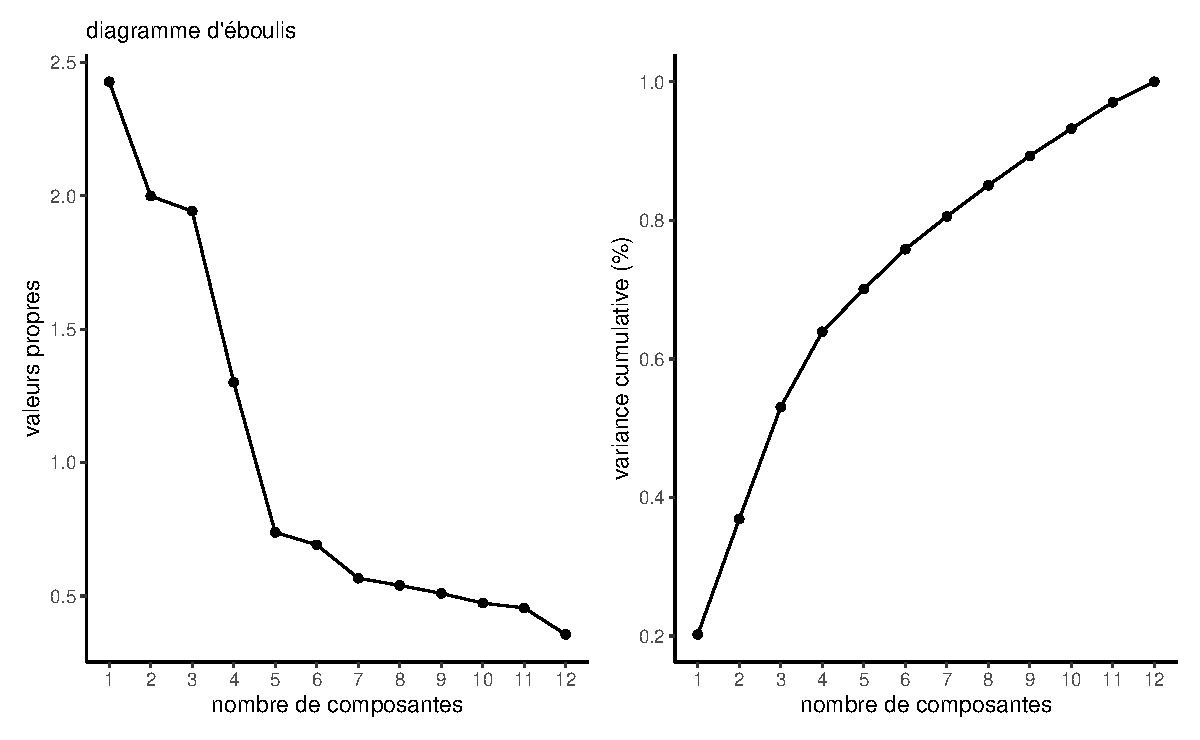
\includegraphics[width=0.7\textwidth,height=\textheight]{./02-analysefactorielle_files/figure-pdf/fig-screeplot-1.pdf}

}

\caption{\label{fig-screeplot}Diagramme d'éboulis (gauche) représentant
la variance des composantes principales (en ordonnée) en fonction du
nombre composantes principales (en abscisse). Variance cumulative en
fonction du nombre de composantes principales (droite).}

\end{figure}

\hypertarget{formulation-mathuxe9matique}{%
\subsection{Formulation
mathématique}\label{formulation-mathuxe9matique}}

Ce complément d'information est optionnel.

Mathématiquement, le problème de l'analyse en composantes principales
revient à calculer la décomposition en valeurs propres et vecteurs
propres de la matrice de covariance
\(\mathsf{Co}(\boldsymbol{X})=\boldsymbol{\Sigma}\). On peut écrire
\begin{align*}
\boldsymbol{\Sigma} = \boldsymbol{Q}\boldsymbol{\Lambda}\boldsymbol{Q}^\top
\end{align*} où
\(\boldsymbol{\Lambda} = \mathrm{diag}\{\lambda_1, \ldots, \lambda_p\}\)
est une matrice diagonale contenant les valeurs propres en ordre
décroissant (\(\lambda_1 \geq \cdots \geq \lambda_p > 0\)) et
\(\boldsymbol{Q}\) est une matrice carrée \(p \times p\) orthogonale
contenant les vecteurs propres. La meilleure approximation de rang
\(k \leq p\) de \(\boldsymbol{\Sigma}\) est obtenue en spécifiant
\begin{align*}
\widetilde{\boldsymbol{\Sigma}}_k = \sum_{j=1}^k \lambda_j \boldsymbol{q}_j\boldsymbol{q}_j^\top,
\end{align*} une combinaison des vecteurs propres
\(\boldsymbol{q}_1, \ldots, \boldsymbol{\gamma}_k \in \mathbb{R}^p\) non
corrélés.

\hypertarget{analyse-factorielle-exploratoire-1}{%
\section{Analyse factorielle
exploratoire}\label{analyse-factorielle-exploratoire-1}}

Si le bigramme a permis de faire ressortir quelques orientations
communes, on aimerait aller plus loin dans notre exploration. On
considère encore une fois la matrice de covariance associée avec \(p\)
variables explicatives \(X_1, \ldots, X_p\): le modèle d'analyse
factorielle cherche à décrire cette dernière en fonction d'un plus petit
nombre de paramètres.

Conceptuellement, le modèle d'analyse factorielle suppose qu'on peut
regrouper les variables explicatives numériques (parfois avec quelques
variables binaires) à l'aide de concepts communs appelés facteurs.
Certaines variables explicatives devraient donc idéalement être
fortements corrélées entre elles. Le choix des variables est dicté par
le bon sens: on inclut dans le modèle des variables qui peuvent
logiquement être associée, par exemple des items de questionnaires
excluant les données sociodémographiques.

Le modèle d'analyse factorielle fait l'hypothèse que les variables
dépendent linéairement d'un plus petit nombre \(m\) de variables
aléatoires, \(F_1, \ldots, F_m\), appelées facteurs communs. Cette
relation n'est pas parfaite, aussi on inclut \(p\) termes d'aléas
\(\varepsilon_1, \ldots, \varepsilon_p\), de moyenne zéro et de variance
\(\mathsf{Va}(\varepsilon_i)=\psi_i\) (\(i=1, \ldots, p\)). À des fins
d'identifiabilité, on suppose que les aléas ne sont pas corrélées aux
facteurs \(F\) et entre elles et que les facteurs \(F_1, \ldots, F_m\)
ont une moyenne nulle et une variance unitaire, donc
\(\mathsf{E}(F_i)=0\) et \(\mathsf{Va}(F_i)=1\) (\(i=1, \ldots, p\)).

Le modèle d'analyse factorielle s'écrit \begin{align*}
\boldsymbol{X} &= \boldsymbol{\mu} + \boldsymbol{\Gamma}\boldsymbol{F} + \boldsymbol{\varepsilon},
\end{align*} ou si on écrit le système ligne par ligne, \begin{align*}
X_1 &= \mu_1 + \gamma_{11}F_1 + \gamma_{12} F_2 + \cdots + \gamma_{1m}F_m + \varepsilon_1\\
X_2 &= \mu_2 + \gamma_{21}F_1 + \gamma_{22} F_2 + \cdots + \gamma_{2m}F_m + \varepsilon_2\\
&\vdots \\
X_p &= \mu_p + \gamma_{p1}F_1 + \gamma_{p2} F_2 + \cdots + \gamma_{pm}F_m + \varepsilon_p, 
\end{align*} où \(\mu_i\) est l'espérance (moyenne théorique) de la
variable aléatoire \(X_i\), où \(\boldsymbol{\Gamma}\) est une matrice
\(p \times m\) avec éléments \(\gamma_{ij}\), qui reprsentent le
chargement de la variable \(X_i\) sur le facteur \(F_j\)
(\(i=1, \ldots, p\); \(j=1, \ldots, m\)).

Les espérances (\(\mu_i\)), les chargements (\(\gamma_{ij}\)) et les
variances (\(\psi_i\)) sont des quantités fixes, mais inconnues, tandis
que les facteurs communs (\(F_i\)) et les aléas (\(\varepsilon_i\)) sont
des variables aléatoires non observables.

Selon ce modèle, on obtient \begin{align*}
\mathsf{Va}(\boldsymbol{X}) &= \boldsymbol{\Gamma}\mathsf{Va}(\boldsymbol{F})\boldsymbol{\Gamma}^\top + \mathsf{Va}(\boldsymbol{\varepsilon})\\
& = \boldsymbol{\Gamma}\boldsymbol{\Gamma}^\top + \mathrm{diag}(\boldsymbol{\psi}).
\end{align*} Les éléments diagonaux de cette matrice sont
\(\mathsf{Va}(X_j) = \sum_{l=1}^k \gamma_{jl}^2 + \psi_j\): on appelle
\textbf{communalité} le terme \(h_j = \sum_{l=1}^k \gamma_{jl}^2\), qui
représente la proportion de variance totale de \(X_j\) due à la
corrélation entre les facteurs. Le terme \(\psi_j\) est dénommé
\textbf{unicité}.

Si les variables ont été préalablement standardisées de telle sorte que
\(\mathsf{E}(X_i)=0\) et \(\mathsf{Va}(X_i)=1\) (ce qui revient à
utiliser la matrice de corrélation des observations dans l'analyse),
alors \(\mathsf{Cor}(X_i, F_j)=\gamma_{ij}\), c'est-à-dire, le
chargement de la variable \(X_i\) sur le facteur \(F_j\) est le
coefficient de corrélation entre les deux.

Sans aucune contrainte sur le modèle, la matrice de covariance de
\(X_1, \ldots, X_p\) possède \(p(p+1)/2\) paramètres, soit \(p\)
variances et \(p(p-1)/2\) termes de corrélation. Avec le modèle
d'analyse factorielle, on suppose que l'on peut décrire cette structure
en utilisant seulement \(p(m+1) - m(m-1)/2\) paramètres\footnote{Soit
  \(p\) variances spécifiques et \(pm\) chargements, moins les
  contraintes de diagonalisation dues à l'invariance du modèle à des
  rotations orthogonales.}. Par exemple, avec \(p=50\) variables
explicatives et \(m=6\) facteurs, on essaie de décrire la structure de
covariance à l'aide de 350 paramètres au lieu de 1275.

Pour faire une analyse factorielle, la taille d'échantillon devrait être
quand même conséquente: le nombre d'entrées dans la base de données est
\(np\) et ce nombre représente la quantité d'unités (information)
disponible pour estimer les covariances. Plusieurs références suggèrent
d'avoir une taille d'échantillon entre cinq et 20 fois le fois le nombre
de variables, ou bien un nombre minimal de 100 à 1000 observations. Des
études de simulations suggèrent que la taille critique dépend des
paramètres, communalités, distribution des données, etc. Ces règles du
pouce sont donc essentiellement arbitraires.

Il existe plusieurs méthodes pour extraire les facteurs, c'est-à-dire
pour estimer les paramètres du modèle (les \(\psi_i\) et les
\(\gamma_{ij}\)). Nous allons discuter de deux d'entre elles: la méthode
du maximum de vraisemblance et la méthode des composantes principales.
L'avantage de l'estimation par maximum de vraisemblance est qu'elle
permet l'utilisation de critères d'information et de statistiques de
tests pour guider le choix du nombre de facteurs, en supposant toutefois
la normalité des facteurs et des aléas.

\hypertarget{rotation-des-facteurs}{%
\subsection{Rotation des facteurs}\label{rotation-des-facteurs}}

Dans le modèle d'analyse factorielle, on peut montrer que, lorsqu'il y a
deux facteurs ou plus, il existe plusieurs configurations de facteurs
qui donnent la même structure de covariance. En fait, les chargements
peuvent seulement être déterminés à une transformation orthogonale
près\footnote{Une transformation orthogonale est une transformation qui
  préserve le produit scalaire; elle préserve ainsi toutes les distances
  et les angles entre deux vecteurs.}. Si les chargements provenant
d'une méthode d'extraction des facteurs ne sont pas uniques, la matrice
de corrélation estimée par le modèle est par contre unique.

Il existe plusieurs techniques de rotation de facteurs. Le but de ces
techniques est d'essayer de trouver une solution qui fera en sorte que
les facteurs seront facilement interprétables. La méthode la plus
utilisée est la méthode \textbf{varimax}: elle produit une configuration
de chargement en maximisant la variance de la somme des carrés des
chargements pour les \(m\) facteurs.

La méthode varimax tend à produire une configuration de facteurs tel que
les chargements de chaque variable sont dispersés (des chargements
élevés positifs ou négatifs et d'autres presque nuls). Il est conseillé
de toujours tenter d'interpréter la solution avec une rotation varimax.
Si ce n'est pas suffisamment clair, il existe d'autres méthodes de
rotation dont certaines (les rotations de type oblique) permettent la
présence de corrélation entre les facteurs.

\hypertarget{estimation-par-la-muxe9thode-des-composantes-principales}{%
\subsubsection{Estimation par la méthode des composantes
principales}\label{estimation-par-la-muxe9thode-des-composantes-principales}}

La façon la plus simple d'estimer les chargements est d'utiliser la
méthode des composantes principales en prenant comme estimation
\begin{align*}
\widehat{\boldsymbol{\Gamma}} = \boldsymbol{Q}_{1:m} \mathrm{diag}(\lambda_1^{1/2}, \ldots, \lambda_m^{1/2}),\end{align*}
où \(\lambda_j\) est la \(j\)e plus grande valeur propre de
\(\boldsymbol{S}\), la matrice de covariance empirique, et
\(\boldsymbol{Q}_{1:m}\) est la sous-matrice formée par les \(m\)
premières colonnes de \(\boldsymbol{Q}\). le vecteur propre associé. On
peut estimer les variances des aléas à travers \begin{align*}
\widehat{\boldsymbol{\psi}} = \mathrm{diag}\left(\mathbf{S} - \widehat{\boldsymbol{\Gamma}}\widehat{\boldsymbol{\Gamma}}^\top\right).
\end{align*} L'avantage de cette approche est que l'on peut utiliser la
même décomposition en valeurs propres et vecteurs propres pour chaque
valeur de \(m\): seule la rotation dépend de la dimension choisie. La
solution est également toujours valide avec la garantie que
\(\widehat{\psi}_j>0\). On peut utiliser la discussion de la
Section~\ref{sec-acp-choix} pour choisir le nombre de variables.

\begin{Shaded}
\begin{Highlighting}[]
\CommentTok{\# Décomposition valeurs propres/vecteurs propres}
\NormalTok{decompo }\OtherTok{\textless{}{-}} \FunctionTok{eigen}\NormalTok{(}\FunctionTok{cor}\NormalTok{(factor))}
\CommentTok{\# Extraire les valeurs propres}
\NormalTok{valpropres }\OtherTok{\textless{}{-}}\NormalTok{ decompo}\SpecialCharTok{$}\NormalTok{values}
\CommentTok{\# Critère de Kaiser}
\NormalTok{ckaiser }\OtherTok{\textless{}{-}} \FunctionTok{sum}\NormalTok{(valpropres }\SpecialCharTok{\textgreater{}} \DecValTok{1}\NormalTok{)}
\CommentTok{\# Extraire les premiers vecteurs propres}
\NormalTok{Gamma\_est }\OtherTok{\textless{}{-}}\NormalTok{ decompo}\SpecialCharTok{$}\NormalTok{vectors[,}\FunctionTok{seq\_len}\NormalTok{(ckaiser)] }\SpecialCharTok{\%*\%}
  \FunctionTok{diag}\NormalTok{(}\FunctionTok{sqrt}\NormalTok{(valpropres[}\FunctionTok{seq\_len}\NormalTok{(ckaiser)]))}
\CommentTok{\# Solution (chargements) avec rotation varimax}
\NormalTok{facto\_cp }\OtherTok{\textless{}{-}} \FunctionTok{varimax}\NormalTok{(Gamma\_est)}
\end{Highlighting}
\end{Shaded}

\hypertarget{estimation-par-maximum-de-vraisemblance}{%
\subsubsection{Estimation par maximum de
vraisemblance}\label{estimation-par-maximum-de-vraisemblance}}

Si on suppose que les aléas et les facteurs suivent des lois
Gaussiennes, alors on peut obtenir une forme explicite pour la fonction
de vraisemblance de la matrice de covariance. L'estimation des
paramètres requiert une optimisation numérique qui est souvent difficile
et qui mène parfois à des solutions paradoxales. On obtient un cas de
quasi-Heywood quand \(h_j=1\) pour une variable \(j\), (on parle de cas
de Heywood si \(h_j > 1\)). Si on modélise des variables explicatives
centrées réduites, \(\mathsf{Va}(X_j)=1\), d'où un problème
d'interprétation car le terme \(\psi_j\) serait nul (cas de
quasi-Heywood) ou négatif (cas de Heywood) alors même que ce terme
représente la variance du \(j\)e aléa. Les cas de quasi-Heywood ont
plusieurs causes, lesquelles sont listées dans la
\href{https://support.sas.com/documentation/cdl/en/statug/63033/HTML/default/viewer.htm\#statug_factor_sect022.htm}{documentation
\textbf{SAS}}. Souvent, c'est dû à l'utilisation d'un trop petit ou trop
grand nombre de facteurs ou une taille d'échantillon trop petite, etc.
Cela complique l'interprétation et nous amène à questionner la validité
du modèle d'analyse factorielle comme simplification de la structure de
covariance.

Les chargements estimés pour la solution à quatre facteurs, suite à la
rotation varimax, sont obtenus avec le code suivant:

\begin{Shaded}
\begin{Highlighting}[]
\CommentTok{\# Ajuster le modèle factoriel par maximum de vraisemblance}
\NormalTok{fa4 }\OtherTok{\textless{}{-}} \FunctionTok{factanal}\NormalTok{(}\AttributeTok{x =}\NormalTok{ factor, }
                \AttributeTok{factors =}\NormalTok{ 4L)}
\CommentTok{\# Imprimer les chargements en omettant les valeurs inférieures à 0.3}
\FunctionTok{print}\NormalTok{(fa4}\SpecialCharTok{$}\NormalTok{loadings, }
      \AttributeTok{cutoff =} \FloatTok{0.3}\NormalTok{)}
\end{Highlighting}
\end{Shaded}

\begin{table}

\caption{\label{tbl-factanal4}\textbf{?(caption)}}\begin{minipage}[t]{\linewidth}
\subcaption{\label{tbl-factanal4-1}}

{\centering 

\begin{tabu} to \linewidth {>{\raggedright}X>{\raggedleft}X>{\raggedleft}X>{\raggedleft}X>{\raggedleft}X}
\toprule
  & F1 & F2 & F3 & F4\\
\midrule
x1 &  &  &  & 99\\
x2 &  &  & 67 & \\
x3 &  & 75 &  & \\
x4 & 71 &  &  & \\
x5 &  &  &  & 37\\
\addlinespace
x6 &  & 51 &  & \\
x7 &  &  & 75 & \\
x8 & 79 &  &  & \\
x9 &  & 63 &  & \\
x10 &  &  & 66 & \\
\addlinespace
x11 & 71 &  &  & \\
x12 &  & 61 &  & \\
\bottomrule
\end{tabu}

}

\end{minipage}%

\end{table}

On constate à la lecture du Tableau~\ref{tbl-factanal4} des chargements
que le chargement associé à la première variable est de 0.992 pour le
facteur 4: cela correspondrait à un facteur avec une corrélation de
presque un, donc \(F_4 \approx X_1\). Le modèle obtenu avec la méthode
du maximum de vraisemblance n'est donc pas adéquat puisque
l'optimisation a convergée vers un cas de quasi-Heywood. Pour
diagnostiquer le tout, on peut aussi analyser les valeurs d'unicité: la
minimum de \texttt{min(fa4\$uniqueness)} est 0.005, ce qui correspond à
la tolérance de l'algorithme (valeur minimale permise dans
l'optimisation), voir \texttt{?factanal}. On retourne à la planche à
dessin en réduisant le nombre de variables.

En général, on associe une variable à un groupe (facteur) si son
chargement est supérieur à 0.3 (en valeur absolue), ce qui donne

\begin{itemize}
\tightlist
\item
  Facteur 1: \(X_4\), \(X_8\) et \(X_{11}\)
\item
  Facteur 2: \(X_3\), \(X_6\), \(X_9\) et \(X_{12}\)
\item
  Facteur 3: \(X_2\), \(X_7\) et \(X_{10}\)
\item
  Facteur 4: \(X_1\) et \(X_5\).
\end{itemize}

Ces facteurs sont interprétables:

\begin{itemize}
\tightlist
\item
  Le facteur 1 représente l'importance accordée au service.
\item
  Le facteur 2 représente l'importance accordée aux produits.
\item
  Le facteur 3 représente l'importance accordée à la facilité de
  paiement.
\item
  Le facteur 4 représente l'importance accordée aux prix.
\end{itemize}

Dans cet exemple, les choses se sont bien passées et le nombre de
facteurs que nous avons spécifié semble être adéquat (hormis le cas de
quasi-Heywood), mais ce n'est pas toujours aussi évident. Il est utile
d'avoir des outils pour guider le choix du nombre de facteurs.

\hypertarget{choix-du-nombre-de-facteurs}{%
\subsection{Choix du nombre de
facteurs}\label{choix-du-nombre-de-facteurs}}

Il existe différentes méthodes pour se guider dans le nombre de
facteurs, \(m\), à utiliser. Cependant, le point important à retenir est
que, peu importe le nombre choisi, il faut que les facteurs soient
\textbf{interprétables}. Par conséquent, les méthodes qui suivent ne
devraient servir que de guide et non pas être suivies aveuglément. La
méthode du maximum de vraisemblance que nous avons utilisée dans
l'exemple possède l'avantage de fournir trois critères pour choisir le
nombre de facteurs appropriés. Ces critères sont:

\begin{itemize}
\tightlist
\item
  le critère d'information d'Akaike (AIC)
\item
  le critère d'information bayésien de Schwarz (BIC)
\item
  le test du rapport de vraisemblance pour l'hypothèse nulle que le
  modèle de corrélation décrit le modèle factoriel avec \(m\) facteurs
  est adéquat, contre l'alternative qu'il n'est pas adéquat.
\end{itemize}

Les critères d'information servent à la sélection de modèles; ils seront
traités plus en détail dans les chapitres qui suivent. Pour l'instant,
il est suffisant de savoir que le modèle avec la valeur du critère AIC
(ou BIC) la plus petite est considéré le « meilleur » (selon ce
critère).

Le paquet \texttt{hecmulti} contient des méthodes pour extraire la
log-vraisemblance, les critères d'information pour un modèle d'analyse
factorielle (objet de classe \texttt{factanal}). On peut extraire la
valeur-\(p\) pour le test du rapport de vraisemblance comparant le
modèle à 12 variables (corrélation empirique) avec le modèle simplifié
obtenu en utilisant quatre facteurs: une valeur-\(p\) supérieur à un
seuil prédéfini (typiquement \(\alpha=0.05\)) indique que la
simplification est adéquate puisqu'on ne rejette pas l'hypothèse nulle.
La sortie suivante dans le Tableau~\ref{tbl-emvcrit} présente les
diagnostics du modèle en fonction du nombre de facteurs pour les modèles
ajustés selon la méthode du maximum de vraisemblance.

\begin{Shaded}
\begin{Highlighting}[]
\FunctionTok{library}\NormalTok{(hecmulti)}
\FunctionTok{ajustement\_factanal}\NormalTok{(}
    \AttributeTok{covmat =} \FunctionTok{cov}\NormalTok{(factor),}
    \AttributeTok{factors =} \DecValTok{1}\SpecialCharTok{:}\DecValTok{5}\NormalTok{,}
    \AttributeTok{n.obs =} \FunctionTok{nrow}\NormalTok{(factor))}
\end{Highlighting}
\end{Shaded}

\begin{table}

\caption{\label{tbl-emvcrit}\textbf{?(caption)}}\begin{minipage}[t]{\linewidth}
\subcaption{\label{tbl-emvcrit-1}}

{\centering 

\begin{tabu} to \linewidth {>{\raggedright}X>{\raggedleft}X>{\raggedleft}X>{\raggedleft}X>{\raggedright}X>{\raggedleft}X>{\raggedleft}X}
\toprule
  & k & AIC & BIC & valeur-p & npar & heywood\\
\midrule
1 & 1 & 2267 & 2346 & < 2e-16 & 24 & 0\\
2 & 2 & 2138 & 2253 & < 2e-16 & 35 & 0\\
3 & 3 & 2017 & 2166 & 0.09604 & 45 & 0\\
4 & 4 & 2003 & 2181 & 0.97262 & 54 & 1\\
5 & 5 & 2013 & 2217 & 0.97445 & 62 & 1\\
\bottomrule
\end{tabu}

}

\end{minipage}%

\end{table}

Le nombre de facteurs à utiliser selon le AIC est 4, versus 3 selon le
BIC. Le nombre mimimal de critères selon le test du rapport de
vraisemblance est NA. Ainsi, on retient la solution à trois facteurs
dans tous les cas: cette adéquation entre les critères est l'exception
plutôt que la règle.

Il faut garder en tête que l'estimation par maximum de vraisemblance du
modèle d'analyse factorielle est très sensible à l'initialisation: on
peut aussi parfois obtenir des valeurs différentes selon les logiciels.
Cette fragilité, couplée à la haute fréquence de cas de Heywood, fait en
sorte que je préfère utiliser la méthode des composantes principales
pour l'estimation.

On peut considérer le modèle avec trois facteurs: les chargements (après
rotation varimax) sont données dans le Tableau~\ref{tbl-factanal3}

\begin{table}

\caption{\label{tbl-factanal3}\textbf{?(caption)}}\begin{minipage}[t]{\linewidth}
\subcaption{\label{tbl-factanal3-1}}

{\centering 

\begin{tabu} to \linewidth {>{\raggedright}X>{\raggedleft}X>{\raggedleft}X>{\raggedleft}X}
\toprule
  & F1 & F2 & F3\\
\midrule
x1 &  &  & \\
x2 &  &  & 67\\
x3 &  & 76 & \\
x4 & 71 &  & \\
x5 &  &  & \\
\addlinespace
x6 &  & 50 & \\
x7 &  &  & 75\\
x8 & 79 &  & \\
x9 &  & 63 & \\
x10 &  &  & 67\\
\addlinespace
x11 & 72 &  & \\
x12 &  & 60 & \\
\bottomrule
\end{tabu}

}

\end{minipage}%

\end{table}

Cette solution récupère les trois facteurs \emph{service},
\emph{produits} et \emph{paiement} de la solution précédente à quatre
facteurs. Le facteur \emph{prix} (qui était formé de \(X_1\) et \(X_5\))
n'est plus présent.

On suggère d'utiliser les trois critères découlant de l'utilisation de
la vraisemblance et de déterminer le nombre de facteurs à extraire selon
différents critères avant d'examiner les modèles avec ce nombre de
facteurs et ceux avec un facteur de moins ou de plus. Au final, le plus
important est de pouvoir interpréter raisonnablement les facteurs: la
configuration de facteurs choisie est logique et compréhensible.

\hypertarget{construction-duxe9chelles-uxe0-partir-des-facteurs}{%
\section{Construction d'échelles à partir des
facteurs}\label{construction-duxe9chelles-uxe0-partir-des-facteurs}}

Si le seul but de l'analyse factorielle est de comprendre la structure
de corrélation entre les variables, alors se limiter à l'interprétation
des facteurs est suffisant.

Si par contre, le but est de réduire le nombre de variables pour pouvoir
par la suite procéder à d'autres analyses statistiques, l'analyse
factorielle peut alors servir de guide pour construire de nouvelles
variables (échelles). En supposant que l'analyse factorielle a produit
des facteurs qui sont interprétables et satisfaisants, la méthode de
construction d'échelles la plus couramment utilisée consiste à
construire \(m\) nouvelles variables, une par facteur. Pour un facteur
donné, la nouvelle variable est simplement la moyenne des variables
ayant des chargements élevés sur ce facteur (positifs ou négatifs, mais
de même signe). Une autre méthode, les scores factoriels, sera présentée
plus loin.

Lorsqu'on construit une échelle, il est important d'examiner sa
cohérence interne. Ceci peut être fait à l'aide du coefficient alpha de
Cronbach. Ce coefficient mesure à quel point chaque variable faisant
partie d'une échelle est corrélée avec le total de toutes les variables
pour cette échelle. Plus le coefficient est élevé, plus les variables
ont tendance à être corrélées entre elles. L'alpha de Cronbach est
\begin{align*}
\alpha=\frac{k}{k-1} \frac{S^2-\sum_{i=1}^k S_i^2}{S^2}, 
\end{align*} où \(k\) est le nombre de variables dans l'échelle, \(S^2\)
est la variance empirique de la somme des variables et \(S_i^2\) est la
variance empirique de la \(i\)e variable. En pratique, on voudra que ce
coefficient soit au moins égal à 0, 6 pour être satisfait de la
cohérence interne de l'échelle.

Le paquet \texttt{hecmulti} contient une fonction, \texttt{alpha}, pour
faire l'estimation du \(\alpha\) de Cronbach

\begin{Shaded}
\begin{Highlighting}[]
\CommentTok{\# Création des échelles}
\NormalTok{ech\_service }\OtherTok{\textless{}{-}} \FunctionTok{rowMeans}\NormalTok{(factor[,}\FunctionTok{c}\NormalTok{(}\StringTok{"x4"}\NormalTok{,}\StringTok{"x8"}\NormalTok{,}\StringTok{"x11"}\NormalTok{)])}
\NormalTok{ech\_produit }\OtherTok{\textless{}{-}} \FunctionTok{rowMeans}\NormalTok{(factor[,}\FunctionTok{c}\NormalTok{(}\StringTok{"x3"}\NormalTok{,}\StringTok{"x6"}\NormalTok{,}\StringTok{"x9"}\NormalTok{,}\StringTok{"x12"}\NormalTok{)])}
\NormalTok{ech\_paiement }\OtherTok{\textless{}{-}} \FunctionTok{rowMeans}\NormalTok{(factor[,}\FunctionTok{c}\NormalTok{(}\StringTok{"x2"}\NormalTok{,}\StringTok{"x7"}\NormalTok{,}\StringTok{"x10"}\NormalTok{)])}
\NormalTok{ech\_prix }\OtherTok{\textless{}{-}} \FunctionTok{rowMeans}\NormalTok{(factor[,}\FunctionTok{c}\NormalTok{(}\StringTok{"x1"}\NormalTok{,}\StringTok{"x5"}\NormalTok{)])}

\CommentTok{\# Cohérence interne (alpha de Cronbach)}
\FunctionTok{alphaC}\NormalTok{(factor[,}\FunctionTok{c}\NormalTok{(}\StringTok{"x4"}\NormalTok{,}\StringTok{"x8"}\NormalTok{,}\StringTok{"x11"}\NormalTok{)])}
\FunctionTok{alphaC}\NormalTok{(factor[,}\FunctionTok{c}\NormalTok{(}\StringTok{"x3"}\NormalTok{,}\StringTok{"x6"}\NormalTok{,}\StringTok{"x9"}\NormalTok{,}\StringTok{"x12"}\NormalTok{)])}
\FunctionTok{alphaC}\NormalTok{(factor[,}\FunctionTok{c}\NormalTok{(}\StringTok{"x2"}\NormalTok{,}\StringTok{"x7"}\NormalTok{,}\StringTok{"x10"}\NormalTok{)])}
\FunctionTok{alphaC}\NormalTok{(factor[,}\FunctionTok{c}\NormalTok{(}\StringTok{"x1"}\NormalTok{,}\StringTok{"x5"}\NormalTok{)])}
\end{Highlighting}
\end{Shaded}

\begin{table}

\caption{\label{tbl-alphaCronbach}\textbf{?(caption)}}\begin{minipage}[t]{\linewidth}
\subcaption{\label{tbl-alphaCronbach-1}}

{\centering 

\begin{tabu} to \linewidth {>{\raggedleft}X>{\raggedleft}X>{\raggedleft}X>{\raggedleft}X}
\toprule
service & produit & paiement & prix\\
\midrule
0.781 & 0.718 & 0.727 & 0.546\\
\bottomrule
\end{tabu}

}

\end{minipage}%

\end{table}

Ainsi, les \(\alpha\) de Cronbach sont tous satisfaisants (plus grand
que 0.6) sauf pour le facteur \emph{prix} (0.546). Tout est donc
cohérent. Les échelles provenant des facteurs \emph{service},
\emph{produits} et \emph{paiement}, sont satisfaisantes. Ces facteurs
sont identifiés à la fois dans la solution à quatre, mais aussi dans la
solution à trois facteurs. Le facteur \emph{prix} est celui qui apparaît
en plus dans la solution à quatre facteurs. Il a une interprétation
claire (c'est essentiellement \texttt{x1}), mais son faible alpha ferait
en sorte qu'il serait discutable de travailler avec l'échelle
\emph{prix} dans d'autres analyses (du moins avec selon l'usage habituel
du alpha) plutôt que d'utiliser directement la variable \texttt{x1}.

\hypertarget{compluxe9ments-dinformation}{%
\section{Compléments d'information}\label{compluxe9ments-dinformation}}

\hypertarget{variables-ordinales}{%
\subsection{Variables ordinales}\label{variables-ordinales}}

Théoriquement, une analyse factorielle ne devrait être faite qu'avec des
variables continues. Par contre, en pratique, on l'utilise souvent aussi
avec des variables ordinales (comme pour l'exemple portant sur le
questionnaire) et même avec des variables binaires (0-1).

Dans ce genre de situation, on peut aussi utiliser d'autres mesures
d'associations au lieu du coefficient de corrélation linéaire. Par
exemple, on peut utiliser la corrélation polychorique, qui est une
mesure de corrélation entre deux variables ordinales. La corrélation
tétrachorique correspond au cas spécial de deux variables binaires.

Ma suggestion est d'utiliser la corrélation linéaire ordinaire avec des
variables ordinales (même binaires). Si les résultats ne sont pas
satisfaisants, on peut alors essayer avec d'autres mesures
d'associations.

\hypertarget{autres-muxe9thodes-de-rotation-des-facteurs}{%
\subsection{Autres méthodes de rotation des
facteurs}\label{autres-muxe9thodes-de-rotation-des-facteurs}}

Jusqu'à présent, nous avons utilisé la méthode de rotation orthogonale
varimax. Il existe de nombreuses autres méthodes de rotations
orthogonales fournies dans le paquet \texttt{psych}. Rappelez-vous que
le modèle d'analyse factorielle de base suppose que les facteurs sont
non corrélés. Les rotations de type obliques permettent d'introduire de
la corrélation entre les facteurs: quelquefois, une telle rotation
facilitera davantage l'interprétation des facteurs qu'une rotation
orthogonale. Notez qu'il faut être prudent lorsqu'on utilise une méthode
de rotation oblique car il y aura trois matrices de chargements après
rotation (coefficients de régression normalisés, corrélations
semi-partielles ou corrélations). On suggère l'utilisation de la
première, soit la représentation avec \textbf{coefficients de régression
normalisés}. Il s'agit des coefficients de régression si on voulait
prédire les variables à l'aide des facteurs. Ils indiquent donc à quel
point chaque facteur est associé à chaque variable. Dans le cas d'une
rotation orthogonale, ces trois matrices sont les mêmes et il s'agit de
trois interprétations valides des chargements.

\hypertarget{scores-factoriels}{%
\subsection{Scores factoriels}\label{scores-factoriels}}

Avec les données de l'exemple, en nous basant sur les résultats de
l'analyse factorielle, nous avons créé quatre nouvelles échelles (une
par facteur) que l'on peut calculer pour chaque individu:

\begin{itemize}
\tightlist
\item
  \texttt{service} = \((X_4+X_8+X_{11})/3\),
\item
  \texttt{produit} = \((X_3+X_6+X_9+X_{12})/4\),
\item
  \texttt{paiement} = \((X_2+X_7+X_{10})/3\),
\item
  \texttt{prix} = \((X_1+X_5)/2\).
\end{itemize}

Par exemple, la variable \emph{prix} peut donc être vu comme une
combinaison linéaire des 12 variables où seulement \(X_1\) et \(X_5\)
reçoivent un poids (égal) différent de zéro. Une autre façon de créer de
nouvelles variables consiste à calculer des scores factoriels (un pour
chaque facteur) pour chaque individu à partir de la matrice de données
centrées et réduite \(\mathbf{Z}\) (de telle sorte que la moyenne de
chaque colonne soit 0 et la variance 1). Les score factoriel
\begin{align*}
\widehat{F}_{i, k} &= \left[\mathbf{Z}\mathbf{R}^{-1}\widehat{\boldsymbol{\Gamma}}\right]_{ik}\\&=
\widehat{\beta}_{1, k} z_{i, 1} + \cdots + \widehat{\beta}_{12, k}z_{i, 12}
\end{align*} où \(\widehat{\boldsymbol{\Gamma}}\) est la matrice
\(p \times m\) des chargements, \(\mathbf{R}\) la matrice \(p \times p\)
des corrélation empirique et où \(z_{i, 1}, \ldots, z_{i, 12}\) est la
\(i\)e ligne (observation) de \(\mathbf{Z}\). La matrice \(p \times m\)
de coefficients
\(\boldsymbol{\beta} = \mathbf{R}^{-1}\widehat{\boldsymbol{\Gamma}}\).

Ainsi, chacune des 12 variables originales contribue au calcul du score
factoriel. Les variables ayant des chargements plus élevés sur ce
facteur auront tendance à avoir des poids (\(\widehat{\gamma}\)) plus
élevés. Par contre, les scores factoriels ne sont pas uniques car ils
dépendent des chargements utilisés (et donc à la fois de la méthode
d'estimation et de la méthode de rotation). On peut également utiliser
les scores factoriels au lieu des 12 variables originales dans des
analyses subséquentes. Il est suggéré d'utiliser les nouvelles variables
(échelles) obtenues en faisant les moyennes des variables identifiées
comme faisant partie de chaque facteur pour les raisons suivantes:

\begin{itemize}
\tightlist
\item
  l'interprétation des scores factoriels est moins claire (chaque
  facteur dépend de toutes les variables)
\item
  les scores factoriels ne sont pas uniques (ils dépendent de la méthode
  d'estimation et de rotation).
\item
  les coefficients servant au calcul seront différents d'une étude à
  l'autre.
\end{itemize}

\begin{table}

\caption{\label{tbl-scores}\textbf{?(caption)}}\begin{minipage}[t]{\linewidth}
\subcaption{\label{tbl-scores-1}}

{\centering 

\begin{tabu} to \linewidth {>{\raggedright}X>{\raggedleft}X>{\raggedleft}X>{\raggedleft}X>{\raggedleft}X}
\toprule
  & facteur 1 & facteur 2 & facteur 3 & facteur 4\\
\midrule
x1 & 0.03 & 0.05 & 0.04 & 1.01\\
x2 & -0.05 & 0.01 & 0.31 & 0.01\\
x3 & 0.01 & 0.45 & -0.02 & 0.01\\
x4 & 0.30 & 0.01 & 0.01 & 0.03\\
x5 & 0.00 & -0.01 & -0.01 & 0.00\\
\addlinespace
x6 & -0.01 & 0.17 & 0.02 & 0.00\\
x7 & -0.01 & -0.02 & 0.44 & 0.02\\
x8 & 0.45 & -0.05 & 0.04 & 0.04\\
x9 & -0.03 & 0.27 & -0.02 & 0.00\\
x10 & 0.02 & 0.01 & 0.30 & 0.02\\
\addlinespace
x11 & 0.30 & 0.00 & -0.07 & 0.02\\
x12 & 0.00 & 0.24 & 0.00 & 0.01\\
\bottomrule
\end{tabu}

}

\end{minipage}%

\end{table}

Les scores factoriels sont obtenus en spécifiant
\texttt{scores\ =\ "regression"} dans les options de la fonction
\texttt{factanal}. Les poids avec le modèle à quatre facteurs sont
rapportés dans le Tableau~\ref{tbl-scores}. On remarque que

\begin{itemize}
\tightlist
\item
  pour le premier facteur, trois variables ont des poids importants
  (\(X_4\), \(X_8\) et \(X_{11}\)). Il s'agit donc d'un facteur très
  proche du facteur \emph{service}.
\item
  pour le deuxième facteur, les variables \(X_3\), \(X_6\), \(X_9\) et
  \(X_{12}\) ont des poids importants. Il s'agit donc d'un facteur très
  proche du facteur \emph{produits}.
\item
  pour le troisième facteur, les variables \(X_2\), \(X_7\), \(X_{10}\)
  ont des poids importants. Il s'agit donc d'un facteur très proche du
  facteur \emph{paiement}.
\item
  pour le quatrième facteur, seule la variable \(X_1\) a un poids
  important. On aurait pu s'attendre à ce que ce soit également le cas
  pour \(X_5\), en lien avec le facteur \emph{prix} --- ce facteur était
  moins clair selon le alpha de Cronbach.
\end{itemize}

Les corrélations entre les échelles (construites avec les moyennes) et
les scores factoriels sont données dans le
Tableau~\ref{tbl-corr-echelles-scores}. On remarque la forte corrélation
entre le score factoriel et les échelles construites avec les moyennes
pour les facteurs \emph{service}, \emph{produits} et \emph{paiement}.
Cela veut dire qu'utiliser les échelles ou les scores factoriels ne
devrait pas faire de différence dans des analyses subséquentes. Par
contre, cette corrélation est plus faible (0.82) pour le facteur
\emph{prix}.

\begin{table}

\caption{\label{tbl-corr-echelles-scores}\textbf{?(caption)}}\begin{minipage}[t]{\linewidth}
\subcaption{\label{tbl-corr-echelles-scores-1}}

{\centering 

\begin{tabu} to \linewidth {>{\raggedright}X>{\raggedleft}X>{\raggedleft}X>{\raggedleft}X>{\raggedleft}X}
\toprule
  & score 1 & score 2 & score 3 & score 4\\
\midrule
échelle 1 & 0.99 & 0.05 & 0.03 & -0.05\\
échelle 2 & 0.05 & 0.98 & 0.03 & -0.04\\
échelle 3 & 0.03 & 0.05 & 0.99 & -0.07\\
échelle 4 & -0.07 & -0.04 & -0.08 & 0.82\\
\bottomrule
\end{tabu}

}

\end{minipage}%

\end{table}

\begin{tcolorbox}[standard jigsaw,title=\textcolor{quarto-callout-tip-color}{\faLightbulb}\hspace{0.5em}{Étapes de l'analyse factorielle exploratoire}, colbacktitle=quarto-callout-tip-color!10!white, bottomrule=.15mm, toptitle=1mm, toprule=.15mm, opacitybacktitle=0.6, bottomtitle=1mm, titlerule=0mm, rightrule=.15mm, colback=white, arc=.35mm, leftrule=.75mm, left=2mm, coltitle=black, colframe=quarto-callout-tip-color-frame, opacityback=0]

\begin{itemize}
\tightlist
\item
  Déterminer les variables à utiliser dans l'analyse
\item
  Vérifier les prérequis
\item
  Sélectionner une méthode d'estimation et extraire les facteurs
\item
  Déterminer le nombre de facteurs
\item
  Effectuer une rotation des facteurs
\item
  Interpréter les facteurs
\item
  Évaluer la validité du modèle
\end{itemize}

\end{tcolorbox}

\begin{tcolorbox}[standard jigsaw,title=\textcolor{quarto-callout-note-color}{\faInfo}\hspace{0.5em}{En résumé}, colbacktitle=quarto-callout-note-color!10!white, bottomrule=.15mm, toptitle=1mm, toprule=.15mm, opacitybacktitle=0.6, bottomtitle=1mm, titlerule=0mm, rightrule=.15mm, colback=white, arc=.35mm, leftrule=.75mm, left=2mm, coltitle=black, colframe=quarto-callout-note-color-frame, opacityback=0]

\begin{itemize}
\tightlist
\item
  La corrélation mesure la force de la dépendance linéaire entre deux
  variables: plus elle est élevée, plus les points s'alignent.
\item
  Si le nombre de variables explicatives \(p\) est conséquent par
  rapport au nombre d'observations \(n\), on a peu d'information
  disponible pour estimer de manière fiable les corrélations.
\item
  Une analyse en composante principales fait une décomposition en
  valeurs propres/vecteurs propres de la matrice de covariance ou de
  corrélation.

  \begin{itemize}
  \tightlist
  \item
    Ces nouvelles variables sont orthogonales (corrélation nulle) entre
    elles.
  \item
    Les composantes principales sont ordonnées en ordre décroissant de
    variance: si on ne conserve que \(k<p\) de variables, on maximise la
    variance expliquée.
  \item
    Le choix du nombre de variables est basé sur des règles du pouce: le
    critère des valeurs propres de Kaiser suggère de prendre autant de
    composantes principales que de variances supérieures à 1.
  \item
    Un bigramme permet de représenter graphiquement les directions des
    variables en fonction des deux premières composantes principales.
  \end{itemize}
\item
  L'analyse factorielle exploratoire fournit un modèle pour la matrice
  de corrélation

  \begin{itemize}
  \tightlist
  \item
    La solution du problème n'est pas unique: on choisit celle qui
    permet de mieux séparer les variables.
  \item
    Seules les variables numériques pour lesquelles on suspecte une
    dimension commune sont incluses dans l'analyse.
  \item
    On doit avoir beaucoup d'observations (au moins 100, 10 fois plus
    que de variables) pour estimer le modèle.
  \item
    On estime le modèle à l'aide de la méthode des composantes
    principales (modèle toujours valide et moins coûteux en calcul, mais
    critères pour la sélection du nombre de facteurs arbitraires) ou du
    maximum de vraisemblance (optimisation numérique avec solutions
    fréquemment problématique, critères d'information pour choix du
    nombre de facteurs).
  \item
    Le nombre de facteurs retenu doit donner des regroupements logiques
    (facteur \emph{wow}).
  \item
    On utilise toujours une rotation orthogonale pour faciliter
    l'interprétation (varimax par défaut).
  \item
    L'interprétation se fait à partir des chargements (corrélation entre
    variables et facteurs).
  \item
    On crée des échelles en prenant la moyenne des variables qui ont un
    chargement élevés en lien avec un facteur donné (de même signe).
  \item
    Les échelles sont cohérentes si le \(\alpha\) de Cronbach est
    supérieur à 0.6, faute de quoi elles sont rejetées.
  \end{itemize}
\end{itemize}

\end{tcolorbox}


\backmatter

\end{document}
